\documentclass[12pt]{report}
\usepackage[a4paper, left=2cm, right=2cm, top=2.5cm, bottom=2.5cm]{geometry}
\usepackage{graphicx}
\usepackage{fontspec}
\usepackage{hyperref}
\usepackage{minted}
\usepackage{tcolorbox}
\usepackage{setspace}
\usepackage{titlesec}
\usepackage{float}
\usepackage{times}
\usepackage[backend=biber,style=numeric,sorting=none]{biblatex}
\usepackage{ragged2e} % per \RaggedLeft, \RaggedRight ecc.

\addbibresource{bibliography.bib}

\definecolor{Titles}{RGB}{159, 6, 167}
\setcounter{secnumdepth}{2}

\geometry{a4paper, margin=2.5cm}

\titleformat{\chapter}
{\color{Titles}\normalfont\Huge\bfseries}
{\thechapter}{1em}{}

\titleformat{\section}
{\color{Titles}\normalfont\LARGE\bfseries}
{\thesection}{1em}{}

\titleformat{\subsection}
{\color{Titles}\normalfont\Large\bfseries}
{\thesubsection}{1em}{}

\tcbuselibrary{listings, skins, breakable}

\newminted[csharp]{csharp}{ 
	fontsize=\small, 
	fontfamily=tt, 
	bgcolor=black, 
	frame=single, 
	framesep=0pt, 
	rulecolor=\color{white}, 
	breaklines=true, 
	breakanywhere=true,
	xleftmargin=0pt,
	xrightmargin=0pt,
	linewidth=\dimexpr\linewidth-1pt\relax,
	texcl=true,
	style=default,
	keywordstyle=\color{cyan}\bfseries, 
	stringstyle=\color{yellow}, 
	commentstyle=\color{green}, 
	showspaces=false, 
	showstringspaces=false
}

\newtcbox{\code}{
	on line,
	box align=base,
	colback=gray!9,
	colframe=gray!1,
	boxrule=0.4pt,
	arc=4pt,
	top=1pt,
	bottom=0.5pt,
	left=1pt,
	right=1pt,
	fontupper=\ttfamily\fontsize{10}{9}\selectfont,
	nobeforeafter,
}

\setmainfont[
ItalicFont  = *Italic,
]{Roboto Light} 
\setmonofont[Scale=.9]{Consolas.ttf}[Path=./]

\setlength{\parindent}{0pt}
\setlength{\parskip}{1em}
\onehalfspacing

\begin{document}
	
	\begin{titlepage}
		\centering
		
		{\Huge Gymnase de Renens\\[0.5em]}
		{\large Travail de Maturité 2024 - 2025}
		
		\vfill
		
		
\includegraphics[width=4cm]{img/rounded_logo_full.png}\\[1em]
		{\Huge Messagyre\\[0.5em]}
		{\large Le gymnase à portée de main}
		
		\vfill
		
		\noindent
		\begin{minipage}[t]{0.48\textwidth}
			\RaggedRight
			Répondant :\\
			Joachim Hugonot
		\end{minipage}%
		\hfill
		\begin{minipage}[t]{0.48\textwidth}
			\RaggedLeft
			Auteur :\\
			Pietro Gravina
		\end{minipage}
	\end{titlepage}
	
	\renewcommand{\contentsname}{Table des matières}
	\tableofcontents
	
	\chapter{Introduction}
	
	Le projet "Messagyre" est né de l’observation d’une série de difficultés rencontrées durant mon expérience au Gymnase de Renens. D’une part, il manquait un système informatique ou une application permettant aux élèves de gérer de manière complète leur année scolaire (devoirs, notes, communications avec les camarades et les professeurs), sans devoir recourir exclusivement à l’agenda papier, déjà dépassé dans de nombreux pays (comme l’Italie, dont je suis originaire). D’autre part, j’ai remarqué l’absence d’un outil de communication plus informel: bien que la suite Microsoft 365 et d’autres instruments soient disponibles, les e-mails sont trop formels et peu pratiques, tandis que les chats d’Outlook et de Teams\supercite{teams} sont peu intuitifs et rarement utilisés.
	
	Pour répondre à ces problématiques, j’ai choisi comme sujet de mon Travail de Maturité la conception, le développement et la réalisation d’une application réunissant dans une seule plateforme toutes les fonctions essentielles à la vie scolaire. "Messagyre" n’est en effet pas seulement une application de messagerie, mais comprend également une section pour la gestion des notes et une autre dédiée aux devoirs, permettant ainsi aux élèves d’avoir tout le nécessaire à portée de main.
	
	Son système de communication est similaire à celui de WhatsApp\supercite{whatsapp}, mais avec une différence fondamentale: il ne nécessite pas le numéro de téléphone du destinataire, car il permet de communiquer simplement en connaissant son prénom (et, si nécessaire, son nom de famille), rendant ainsi les échanges entre étudiants et enseignants beaucoup plus rapides et accessibles. Le nom "Messagyre" provient de la fusion des mots "Messages" et "Gyre" (ce dernier étant lui-même une contraction de Gymnase de Renens).
	
	Je considère ce projet particulièrement intéressant et ambitieux. Bien qu’une application de chat puisse sembler simple à développer au premier abord, il s’agit en réalité d’un projet complexe nécessitant des compétences avancées, tant en programmation qu’en design.
	
	Avant de commencer ce projet, je possédais déjà des connaissances avancées en programmation. Je programme depuis l’âge de huit ou neuf ans, ayant appris en autodidacte plusieurs langages, notamment C\#\supercite{csharp}, Python, Lua, Java, JavaScript\supercite{nodejs} et Dart\supercite{dart}.
	
	Mes premières expériences en communication client-serveur consistaient en de simples échanges de données entre des pages HTML avec des scripts en JavaScript\supercite{nodejs} et un serveur basé sur Node.js\supercite{nodejs}. Cependant, afin de tester la faisabilité de ce projet et de proposer l’idée officiellement à la direction, j’ai développé un premier prototype en utilisant Unity\supercite{visualstudio} comme client et un serveur en Node.js (JavaScript\supercite{nodejs}). Bien que le système fonctionnait, la principale difficulté était d’optimiser la communication entre ces deux langages, très différents dans leur approche.
	
	Après quelques recherches, j’ai découvert qu’il était possible de développer le serveur directement en C\#\supercite{csharp}, en utilisant l’API ASP.NET Core\supercite{aspnetcore} de Microsoft. J’ai donc entièrement réécrit l’application sur Unity\supercite{visualstudio} ainsi que le serveur, améliorant donc la stabilité et l’intégration du système. Pour le développement, j’ai utilisé Visual Studio 2022\supercite{visualstudio}, l’environnement de développement de Microsoft, pour le client ainsi que pour le serveur.
	
	Néanmoins, après avoir avancé avec Unity\supercite{visualstudio}, j’ai constaté que cette plateforme n’était pas idéale pour développer une application mobile de messagerie, principalement à cause des contraintes liées à la gestion de l’interface utilisateur et à la lourdeur de l’environnement pour ce type d’application. J’ai alors décidé de migrer le client vers Flutter\supercite{flutter}, un framework moderne spécialisé dans le développement d’interfaces mobiles performantes et adaptatives. Cette décision m’a permis d’améliorer considérablement l’expérience utilisateur tout en conservant ASP.NET Core\supercite{aspnetcore} pour la partie serveur.
	
	Dans ce document, les différentes phases du projet seront présentées en détail : du contexte initial et de l’analyse des applications existantes, au développement technique du client et du serveur, aux fonctionnalités avancées, aux résultats obtenus et aux difficultés rencontrées tout au long du projet. Enfin, je conclurai par une réflexion personnelle sur le travail accompli et les compétences acquises.
	
	\chapter{Contexte et analyse préliminaire}
	
	\section{Panorama des applications de messagerie}
	
	Les applications de messagerie instantanée occupent aujourd’hui une place centrale dans la communication quotidienne, tant au niveau personnel que professionnel. Des services comme WhatsApp\supercite{whatsapp}, Telegram\supercite{telegram} ou Signal\supercite{signal} permettent des échanges rapides, souvent gratuits, et proposent diverses fonctionnalités telles que les appels vocaux, le partage de fichiers, et la création de groupes.
	
	Ces applications visent à faciliter la communication en temps réel, en garantissant à la fois la simplicité d’utilisation et la sécurité des échanges. Cependant, elles présentent parfois des limites dans le cadre de communications institutionnelles ou spécifiques, comme celles d’un établissement scolaire, où la gestion des utilisateurs et la confidentialité doivent être adaptées, contrairement à Microsoft Teams\supercite{teams} plus orienté vers les usages professionnels et collaboratifs.
	
	\section{Analyse de la concurrence}
	
	Les principales applications concurrentes sur le marché sont WhatsApp\supercite{whatsapp}, Telegram\supercite{telegram}, Signal\supercite{signal} et Microsoft Teams\supercite{teams}. WhatsApp\supercite{whatsapp} est très populaire, mais utilise le numéro de téléphone comme identifiant principal, ce qui peut poser des problèmes de confidentialité. Telegram\supercite{telegram} offre davantage de fonctionnalités avancées, comme des canaux publics et une meilleure gestion de la vie privée, mais nécessite un certain niveau de familiarité technique. Signal\supercite{signal} se concentre sur la sécurité et la confidentialité, avec un chiffrement de bout en bout par défaut. Microsoft Teams\supercite{teams}, intégré à la suite Microsoft 365, permet la communication et la collaboration, mais reste plus formel et moins intuitif pour les échanges informels entre étudiants et enseignants.  
	
	Aucune de ces solutions ne répond parfaitement aux besoins spécifiques d’un environnement scolaire comme le Gymnase de Renens, notamment en termes de facilité d’accès basée uniquement sur le prénom et le nom, sans nécessiter de numéro de téléphone.
	
	\section{Technologies principales impliquées}
	
	Pour le développement de Messagyre, plusieurs technologies clés ont été utilisées tout au long du projet. Pour le client mobile multiplateforme, le framework de Google\supercite{google} Flutter\supercite{flutter} a été choisi, utilisant le langage Dart\supercite{dart}, permettant de créer une interface moderne, fluide et performante sur Android et iOS. Le serveur est développé avec le framework de Microsoft\supercite{microsoft} ASP.NET Core\supercite{aspnetcore} en C\#\supercite{csharp}, garantissant robustesse, performances et facilité de maintenance. Initialement, le backend était développé en Node.js\supercite{nodejs} pour prototyper rapidement les fonctionnalités en temps réel.
	
	La communication entre le client et le serveur utilise HTTP\supercite{http} pour les requêtes classiques (comme l'authentification et la récupération des données) et WebSocket\supercite{websocket} pour la messagerie instantanée en temps réel. Les données des utilisateurs et des messages sont stockées dans une base de données MySQL\supercite{mysql}, initialement hébergée sur Railway\supercite{railway}, puis sur un VPS, c’est-à-dire un ordinateur « à louer » actif en permanence. Le programme backend était également initialement hébergé sur Railway, mais pour des raisons de coût (voir section Hébergement et Budget \ref{hostingandbudget}) il a été déplacé sur Fly.io\supercite{flyio}, pour finalement être hébergé sur le même ordinateur que la base de données.
	
	Pour la gestion locale des données sur l'appareil, comme l'historique des messages, Hive\supercite{hive} est utilisé, une librairie Flutter qui permet de stocker des informations sur le disque dur en imitant une petite base de données. D'autres données plus sensibles, comme les tokens pour l'accès à l'application (voir section Développement du serveur \ref{serverdevelopment}), sont stockées dans Flutter Secure Storage, également une librairie Flutter capable de chiffrer et déchiffrer les données avant de les sauvegarder. Les notifications push sont gérées par Firebase\supercite{firebase}, un ensemble de services web de Google\supercite{google}. L'envoi des emails de vérification utilisait initialement un serveur SMTP\supercite{smtp}, mais à cause de certaines restrictions (voir section Hébergement et Budget \ref{hostingandbudget}) il utilise actuellement les API de Gmail\supercite{gmailapi}, et les photos de profil sont hébergées par Cloudinary\supercite{cloudinary}, un service tiers permettant de stocker des photos accessibles à tous gratuitement.
	
	Pour la conception graphique des icônes et des éléments visuels de l'application, des outils comme Remove.bg\supercite{removebg} ont été utilisés pour supprimer l'arrière-plan, Pixlr E\supercite{pixlre} pour modifier les couleurs et créer certaines icônes, Canva\supercite{canva} et Adobe Express\supercite{adobeexpress} pour des graphismes plus complexes. Enfin, le versionnage du code et la gestion du projet ont été réalisés avec Git\supercite{git} puis publiés sur GitHub\supercite{github}, tandis que le codage s'est déroulé principalement sur Visual Studio\supercite{visualstudio} pour le backend et Visual Studio Code\supercite{vscode} pour le frontend.
	
	
	\chapter{Développement du projet}
	
	\section{Analyse des besoins et spécifications}
	
	L’application Messagyre a été conçue pour répondre à plusieurs besoins fondamentaux, dans le but de faciliter la communication interne au Gymnase de Renens tout en permettant une gestion complète des devoirs et des notes des élèves. L’application assure une authentification sécurisée des utilisateurs, permet l’envoi et la réception de messages texte en temps réel via WebSocket\supercite{websocket}, et gère les profils utilisateurs, incluant la possibilité d’ajouter une photo de profil hébergée sur Cloudinary\supercite{cloudinary} et d’autres informations de contact telles que l’adresse e-mail, le numéro de téléphone ou les liens vers les réseaux sociaux. Messagyre sert également de véritable agenda scolaire, permettant l’ajout de devoirs et de notes, et offre une interface intuitive et accessible même aux utilisateurs moins expérimentés, garantissant une utilisation rapide, agréable et sécurisée, tout en protégeant la confidentialité des communications\supercite{https}.
	
	Le public cible comprend principalement les élèves, mais aussi les enseignants et le personnel du gymnase, avec une attention particulière portée à la facilité d’accès, sans nécessiter l’utilisation d’un numéro de téléphone. Des prototypes initiaux ont été réalisés pour définir la disposition des écrans principaux, tels que la page de connexion et d’inscription, la liste des conversations, la fenêtre de chat et le profil utilisateur, guidant ainsi le développement de l’interface.
	
	Pour permettre le bon fonctionnement de l’application, un backend a été nécessaire, c’est-à-dire un système chargé de gérer les utilisateurs et leurs interactions, y compris toutes les opérations liées aux messages. Pour cela, ASP.NET Core\supercite{aspnetcore}, un framework de Microsoft pour le développement d’applications web en C\#\supercite{csharp}, a été choisi, langage avec lequel je possède une expérience solide. Le backend gère les utilisateurs connectés à la plateforme, leurs informations personnelles comme le nom d’utilisateur, l’adresse e-mail, le mot de passe, la photo 
	
	de profil et les détails du profil public, permet la création de nouveaux comptes et l’accès aux comptes existants, trie les messages et vérifie qu’ils sont correctement reçus par les destinataires. La communication entre le client et le serveur se fait via HTTP\supercite{http} pour les opérations classiques et WebSocket\supercite{websocket} pour la messagerie en temps réel.
	
	Grâce à cette architecture, Messagyre combine sécurité, efficacité et simplicité d’utilisation, répondant de manière complète aux besoins de la vie scolaire numérique.
	
	\section{Développement du client (Flutter)}
	
	La structure de l'application mobile est basée sur le framework Flutter\supercite{flutter}, choisi pour sa capacité à créer des interfaces réactives et multiplateformes à partir d'un seul code source en Dart\supercite{dart}. Flutter permet également de visualiser en temps réel les modifications du code sans avoir à recompiler l'application entière, grâce à la fonction de hot reload, rendant le développement plus simple et rapide par rapport à d'autres systèmes, comme Unity utilisé précédemment.
	
	Pour la persistance locale des données, telles que l'historique des messages et les paramètres de l'utilisateur, les bibliothèques Hive\supercite{hive} et Flutter Secure Storage\supercite{securestorage} sont utilisées, cette dernière servant également à stocker en toute sécurité les mots de passe. Les notifications push sont gérées via Firebase\supercite{firebase}, par lequel le serveur les envoie directement au client, permettant aux utilisateurs de recevoir des mises à jour même lorsque l'application n'est pas active.
	
	L'interface utilisateur a été conçue en suivant le style iOS avec Cupertino, une bibliothèque de composants intégrée à Flutter qui reproduit fidèlement l'apparence et le comportement natif des applications Apple. Ce choix a été fait pour sa modernité et sa cohérence visuelle, offrant une expérience fluide et agréable aux utilisateurs.
	
	La première partie du développement de l'application a été l'implémentation de l'authentification : j'ai créé les pages dédiées à la connexion et à l'inscription, permettant à l'utilisateur de s'identifier une seule fois et d'accéder à l'application. Ensuite, je me suis concentré sur le développement d'une page listant les conversations, suivie d'une page pour chaque conversation. 
	Pour permettre aux utilisateurs de rechercher d'autres utilisateurs avec lesquels échanger des messages, j'ai ajouté une page dédiée, par laquelle l'application envoie une requête HTTP\supercite{http} au serveur qui renvoie une liste de résultats. En cliquant sur l'un des résultats, une page "profil" permet de visualiser les informations de l'utilisateur, telles que son nom d'utilisateur, son surnom, son email scolaire, sa classe et tout ce que cette personne a ajouté à son profil. 
	Une fois la partie principale de "l'application de messagerie" terminée, je me suis concentré sur le développement d'une page pour les notes, avec une liste des branches et leurs moyennes, une sous-page pour visualiser les notes d'une branche spécifique et une autre sous-page pour ajouter une note, avec titre, valeur, branche, groupe d'évaluation et informations supplémentaires telles que la description et les photos du test ou du travail évalué. 
	Enfin, la page pour les devoirs a été la dernière à être développée, avec un calendrier horizontal contenant tous les devoirs ajoutés par l'utilisateur via la sous-page correspondante, où l'on peut choisir la branche, une description, si c'est un devoir noté ou un test. 
	La page des paramètres a été implémentée au fur et à mesure que l'application prenait forme, en ajoutant des options pour modifier son profil, se déconnecter, activer le mode sombre, changer l'arrière-plan des conversations, supprimer les données et personnaliser des composants de l'application tels que le calendrier et les branches.
	
	\section{Développement du serveur (ASP.NET Core)}
	\label{serverdevelopment}
	
	Le serveur backend, c’est-à-dire le programme qui gère toutes les requêtes de l’application, comme l’envoi de messages, la recherche d’autres utilisateurs, etc., a été développé avec \textbf{ASP.NET Core}\supercite{aspnetcore}, un framework open source de Microsoft\supercite{microsoft} pour le développement d’applications web modernes, multiplateformes et hautes performances. J’ai choisi cette technologie pour sa robustesse, ses hautes performances et ma familiarité avec le langage C\#\supercite{csharp}.
	
	La communication en temps réel entre le client et le serveur est basée sur \textbf{WebSocket}\supercite{websocket}, qui permet l’envoi et la réception instantanés des messages. Pour les opérations plus classiques, comme l’authentification, la création ou la modification d’un compte, le serveur expose des \textbf{API REST}\supercite{apirest}. Une API REST (Representational State Transfer) est un ensemble de règles permettant à deux systèmes de communiquer via des requêtes HTTP standard (GET, POST, PUT, DELETE), de manière simple et uniforme, rendant ainsi les interactions entre le client et le serveur plus claires et plus évolutives.
	
	Le système d’authentification reçoit les identifiants saisis par l’utilisateur dans l’application, vérifie s’ils sont valides, et si c’est le cas, renvoie un jeton « \textbf{JSON Web Token (JWT)} »\supercite{http}, c’est-à-dire un texte chiffré contenant diverses informations prouvant que l’utilisateur est autorisé à accéder à l’application, avec une certaine date d’expiration. En plus de ce jeton, un autre est également envoyé au client, moins complexe (il s’agit d’un simple UUID\supercite{uuid}), que j’ai appelé « refresh token », afin de valider et prolonger les sessions des utilisateurs sans devoir redemander leurs identifiants à chaque ouverture de l’application.
	
	La base de données relationnelle \textbf{MySQL}\supercite{mysql} stocke des informations telles que la liste de tous les comptes utilisateurs et une liste de messages dans la « inbox », c’est-à-dire des messages qui n’ont pas encore été remis à leur destinataire, car celui-ci n’a pas été en ligne depuis leur envoi.
	
	Chaque compte dans la base de données contient des informations telles que : le nom, l’adresse e-mail scolaire, le mot de passe chiffré (avec hachage\supercite{bcrypt}), la photo de profil, le jeton d’accès JWT\supercite{jwt}, le refresh token, des informations publiques comme le pseudonyme et la biographie, ainsi que d’autres données nécessaires à certaines fonctionnalités comme les notifications push. Les messages, quant à eux, contiennent le contenu, l’heure d’envoi, l’état de lecture, etc.
	
	La majorité des fonctionnalités sont gérées par le programme que j’ai écrit, sauf quelques exceptions : l’envoi des e-mails de vérification lors de la création d’un compte utilisateur a d’abord été géré par un serveur SMTP\supercite{smtp}, puis par les API de Gmail\supercite{googleapi} ; les photos de profil sont stockées dans une base de données tierce, gérée par Cloudinary\supercite{cloudinary} ; la base de données était initialement hébergée sur Railway\supercite{railway}, mais a ensuite été transférée sur le serveur de mon professeur, \textbf{voir la section Hébergement et budget \ref{hostingandbudget}} ; le programme backend lui-même, tout comme la base de données, a été déplacé plusieurs fois : il fonctionnait d’abord sur Railway\supercite{railway}, puis sur Fly.io\supercite{flyio}, avant d’être finalement transféré sur le serveur de mon professeur.
	
	\section{Fonctionnalités avancées}
	
	Dans Messagyre, plusieurs fonctionnalités avancées ont été intégrées pour améliorer l'expérience utilisateur et la qualité globale de l'application. La gestion des photos de profil permet aux utilisateurs de télécharger une image personnelle qui est automatiquement mise à jour et affichée auprès des autres utilisateurs dès qu'elle est modifiée\supercite{cloudinary}. De plus, il est désormais possible de disposer d'un profil public consultable par les autres utilisateurs, contenant des informations de base telles que le nom, la photo et d'autres détails choisis par l'utilisateur, facilitant ainsi l'identification et l'interaction au sein de la plateforme.
	
	Les notifications push sont entièrement opérationnelles : le serveur envoie aux utilisateurs une alerte immédiate lorsqu'un nouveau message ou une communication importante est reçue, garantissant la réception en temps réel même lorsque l'application n'est pas ouverte au premier plan\supercite{firebase}. En termes de performances, l'application gère efficacement les connexions WebSocket\supercite{websocket} et réduit le nombre d'appels HTTP inutiles\supercite{http}, améliorant ainsi la vitesse et réduisant la consommation de données, ce qui est particulièrement important sur les appareils mobiles avec des connexions instables ou limitées.
	
	Concernant la sécurité, toutes les communications entre le client et le serveur sont chiffrées via HTTPS et des WebSockets sécurisés. Les données envoyées par les utilisateurs sont systématiquement validées côté serveur pour prévenir tout comportement inattendu ou malveillant. Des contre-mesures ont été mises en place pour se protéger contre les attaques courantes telles que les injections SQL, le Cross-Site Scripting (XSS) et les attaques de type Man-in-the-Middle (MITM), conformément aux recommandations de l'\textbf{OWASP}\supercite{owasp}, qui définit les bonnes pratiques pour sécuriser les applications web contre les vulnérabilités et attaques informatiques.
	
	Enfin, une page de débogage a été ajoutée dans les paramètres, permettant aux utilisateurs de vérifier d'éventuels problèmes avec l'application. Cette fonctionnalité est particulièrement utile pour détecter des erreurs qui ne se manifestent pas lors des tests sur émulateur ou sur les appareils de développement, facilitant ainsi le débogage et la résolution rapide des problèmes.
	
	\section{Tests et débogage}
	
	Au début de la phase de développement, les principales difficultés rencontrées concernaient la gestion en temps réel des messages, la synchronisation des horaires d'envoi et de réception, la stabilité des connexions et l'authentification via token (une nouveauté pour moi), résolues grâce à une meilleure gestion de l'état côté client et côté serveur.
	
	Le projet a suivi plusieurs tests pour garantir la fiabilité ainsi qu'une bonne expérience utilisateur de l'application. Les tests les plus fréquents ont été des tests manuels où j'ai fait exécuter l'application sur l'émulateur Android officiel d'Android Studio \supercite{androidstudio} via le débogueur officiel de Flutter dans Visual Studio Code. Grâce à cela, j'ai pu développer une interface graphique propre et agréable à regarder, une accessibilité optimale en déplaçant les différents boutons pour qu'ils soient plus facilement actionnables par les doigts de l'utilisateur, le fonctionnement complet des fondations de l'application et l'exécution correcte des processus non visibles dans l'application elle-même (processus en arrière-plan). D'autres tests ont été réalisés en construisant l'application pour les plateformes spécifiques (Android et iPhone) en utilisant un téléphone physique ; grâce à ces tests, j'ai trouvé plusieurs « failles » qui n'apparaissaient pas sur l'émulateur, telles que des animations graphiques défaillantes, des champs de texte inutilisables, et autres. De plus, j'ai pu tester les notifications push, mais cela avec l'aide de la console Firebase, le service utilisé par le serveur pour les envoyer.
	
	Les tests mentionnés jusqu'ici concernaient uniquement l'application, la partie « client », mais le serveur a également nécessité plusieurs vérifications pour fonctionner correctement. Comme mentionné dans la section \ref{serverdevelopment}, le serveur a été déplacé entre plusieurs plateformes, chacune avec ses propres exigences. Pour vérifier que le serveur répondait correctement, j'ai utilisé le navigateur Chrome \supercite{chrome}, en envoyant des requêtes HTTP \supercite{http} et HTTPS \supercite{https} au serveur via la barre de recherche du navigateur. Pour tous les autres tests, je me suis servi de l'application elle-même, car l'authentification nécessitait de nombreuses requêtes, ainsi qu'une connexion WebSocket, plus longue et complexe à réaliser via un navigateur.
	
	La communication entre le serveur et la base de données MySQL \supercite{mysql} a également été testée, en effectuant plusieurs appels via l'application et un programme externe MySQL Workbench \supercite{mysqlworkbench}, et en vérifiant que les informations étaient correctement enregistrées et qu'aucun problème de données corrompues ne survenait lors de la lecture par le serveur.
	
	\chapter{Résultats obtenus}
	
	\section{État actuel de l'application}
	
	À ce jour, l'application Messagyre fonctionne pleinement dans ses fonctionnalités principales. Les utilisateurs peuvent créer un compte via leur adresse e-mail scolaire, se connecter de manière sécurisée, envoyer et recevoir des messages en temps réel, modifier leur profil et consulter ceux des autres utilisateurs. Le système de messagerie repose sur WebSocket, garantissant une communication fluide et instantanée.
	
	Certaines fonctionnalités secondaires sont encore en cours de développement ou prévues pour les prochaines versions, notamment :
	
	\begin{itemize}
		\item Implémentation des notifications push.
		\item Gestion complète des devoirs et des notes dans les pages « Devoirs » et « Notes » respectivement.
		\item Améliorations graphiques de l’interface utilisateur.
		\item Animations pour rendre l’utilisation de l’application plus agréable.
		\item Possibilité de créer et de rejoindre des groupes de discussion.
		\item Une page dédiée aux annonces et communications officielles (ou non) du gymnase.
	\end{itemize}
	
	\section{Comparaison avec les objectifs initiaux}
	
	Le projet a atteint la majorité des objectifs fixés au départ :
	
	\begin{itemize}
		\item Développer un système de messagerie interne, sécurisé et facile à utiliser.
		\item Permettre une communication simple sans utiliser le numéro de téléphone.
		\item Intégrer des comptes scolaires avec vérification par e-mail.
		\item Implémenter une page pour la gestion des devoirs.
	\end{itemize}
	
	Dans l’ensemble, les résultats obtenus sont très satisfaisants, compte tenu de la complexité technique du projet, du temps disponible et du fait qu’il s’agit d’un développement réalisé entièrement de manière autonome.
	
	\section{Captures d’écran de l’application}
	
	Voici quelques captures d’écran de Messagyre dans son état actuel, accompagnées d’une brève description :
	
	\begin{figure}[H]
		\centering
		\begin{minipage}[t]{0.45\textwidth}
			\centering
			\fbox{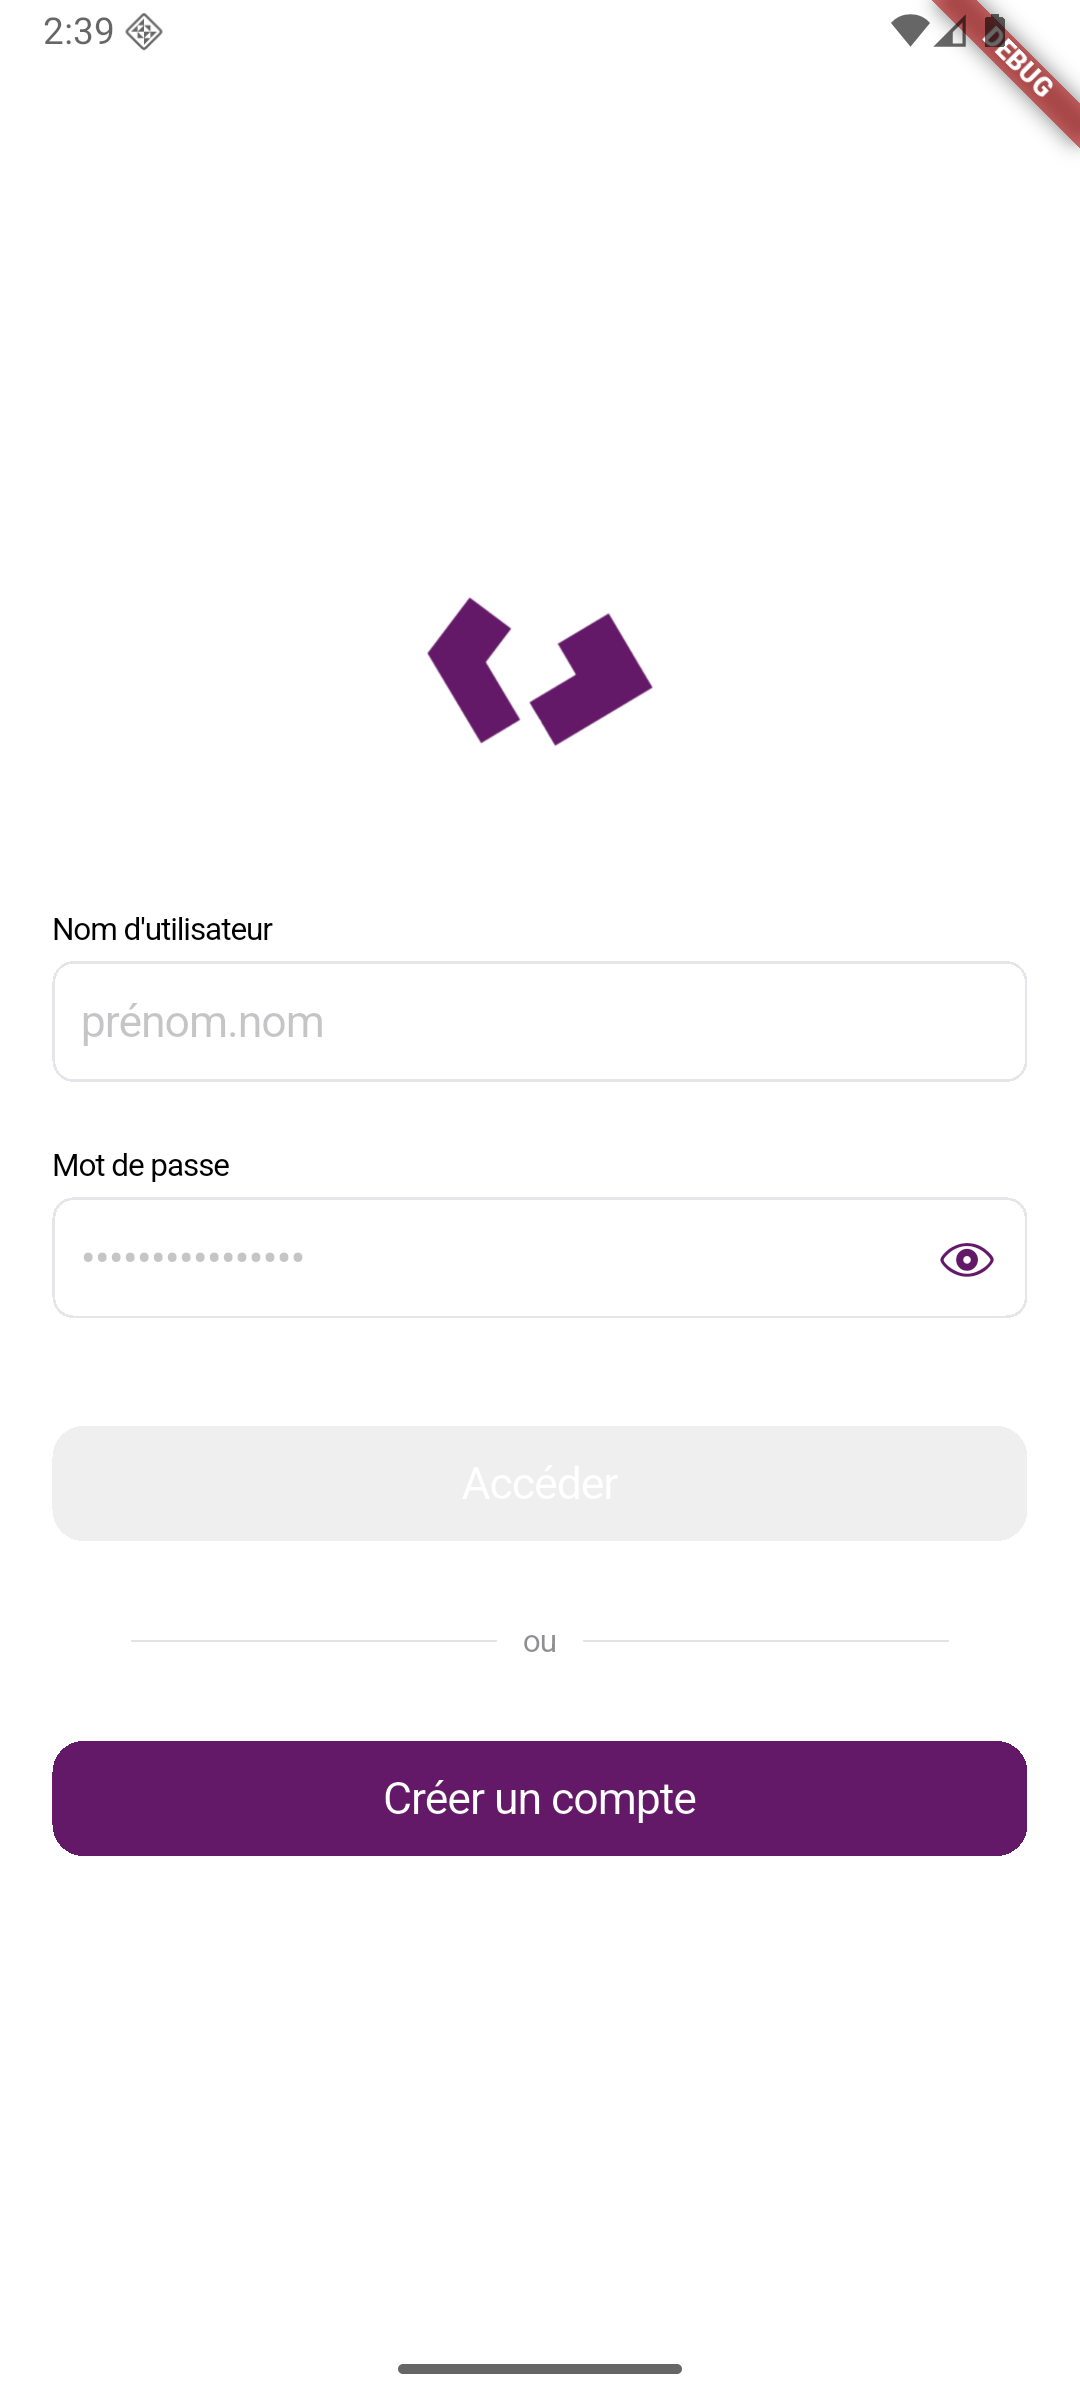
\includegraphics[width=\textwidth]{img/login.png}}
			\caption*{\textbf{Page de connexion} : avec les champs de saisie et le bouton de connexion.}
		\end{minipage}
		\hfill
		\begin{minipage}[t]{0.45\textwidth}
			\centering
			\fbox{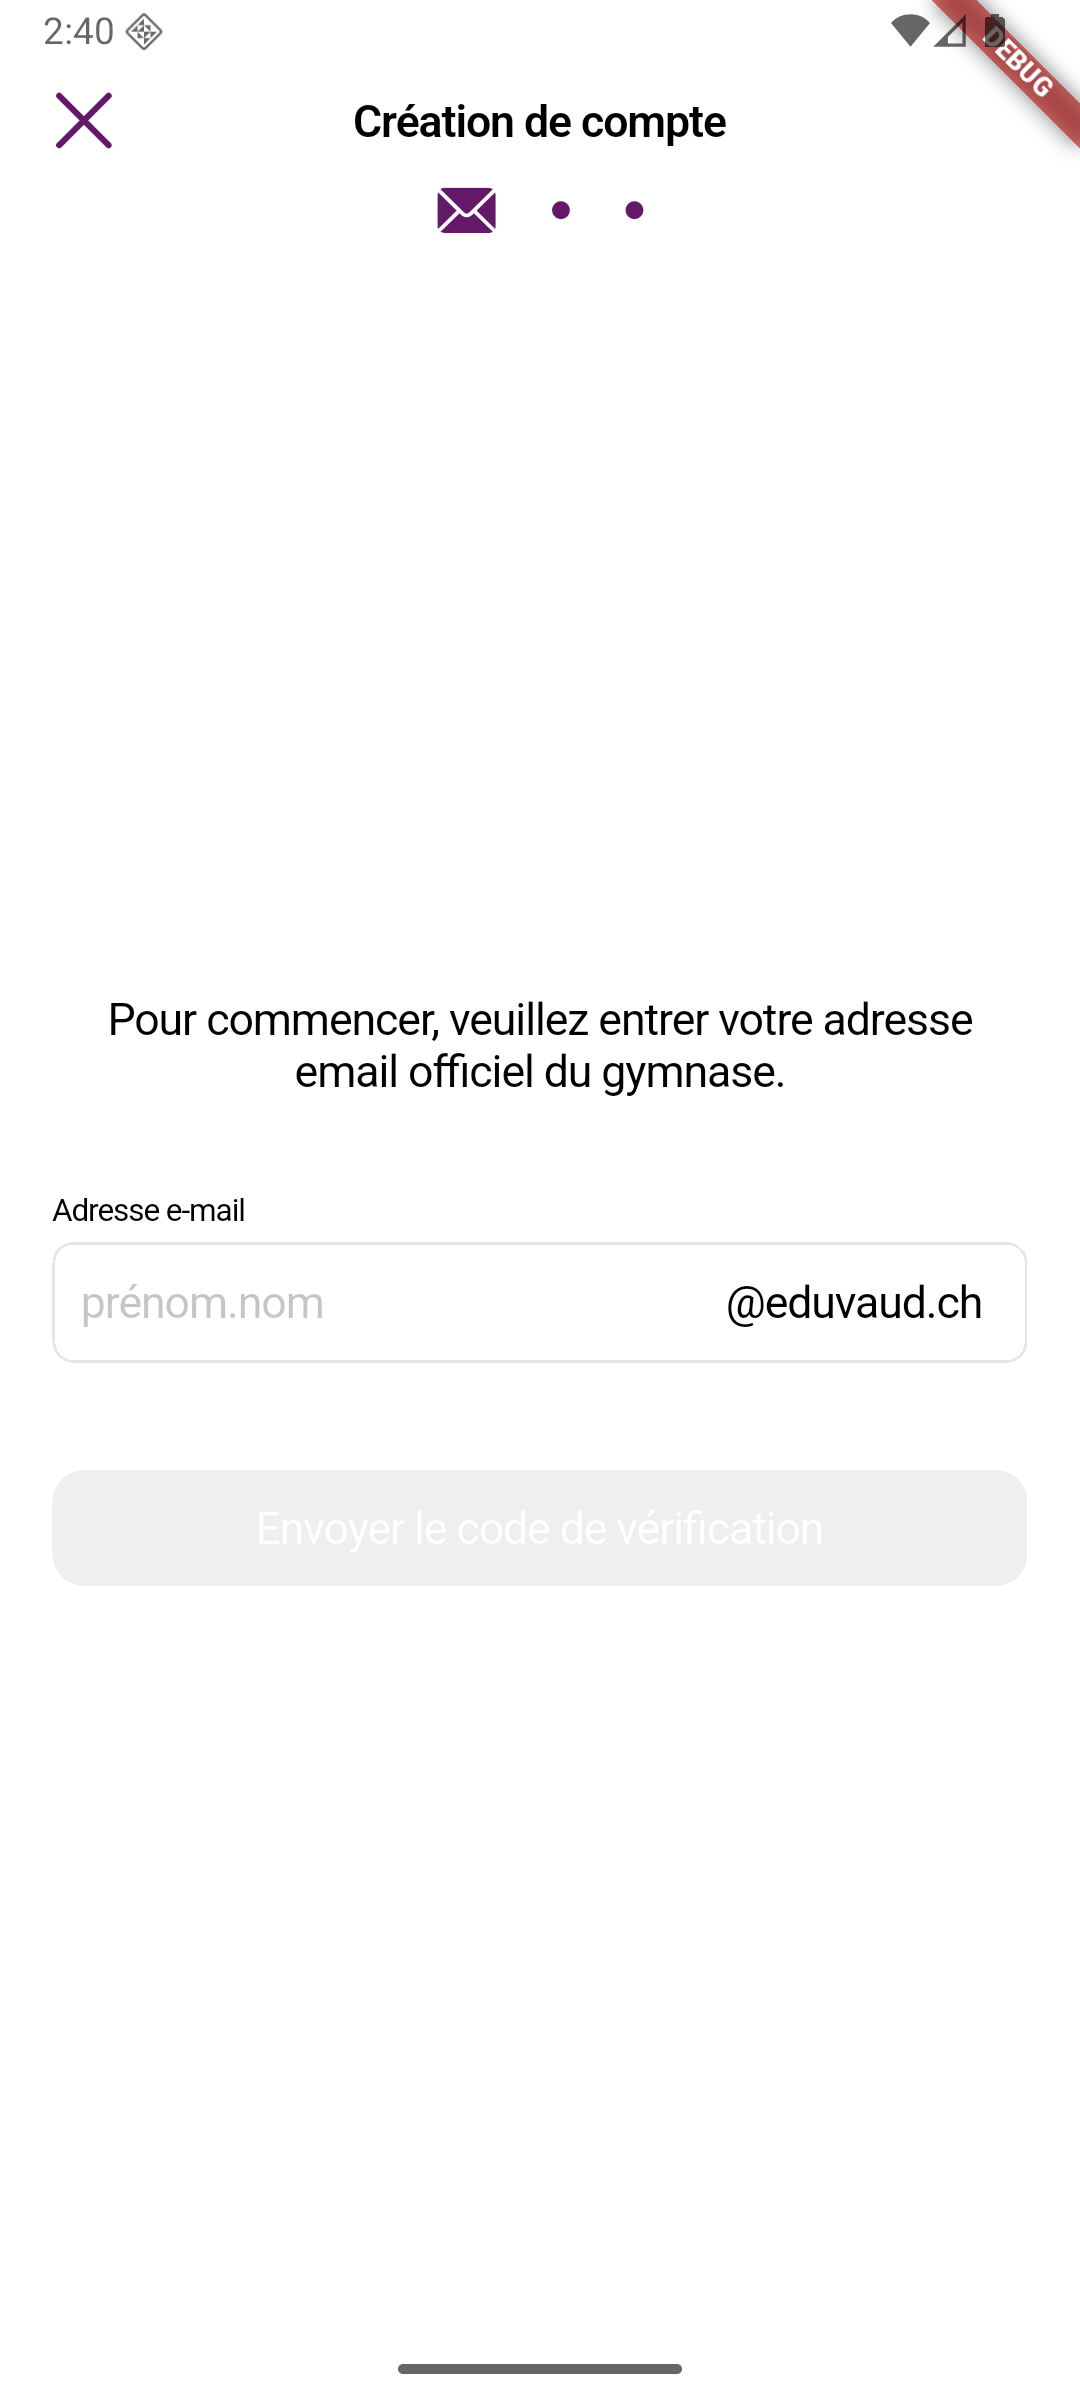
\includegraphics[width=\textwidth]{img/registration_email.png}}
			\caption*{\textbf{Page d'inscription} : formulaire avec vérification de l’adresse e-mail.}
		\end{minipage}
	\end{figure}
	
	\begin{figure}[H]
		\centering
		\begin{minipage}[t]{0.45\textwidth}
			\centering
			\fbox{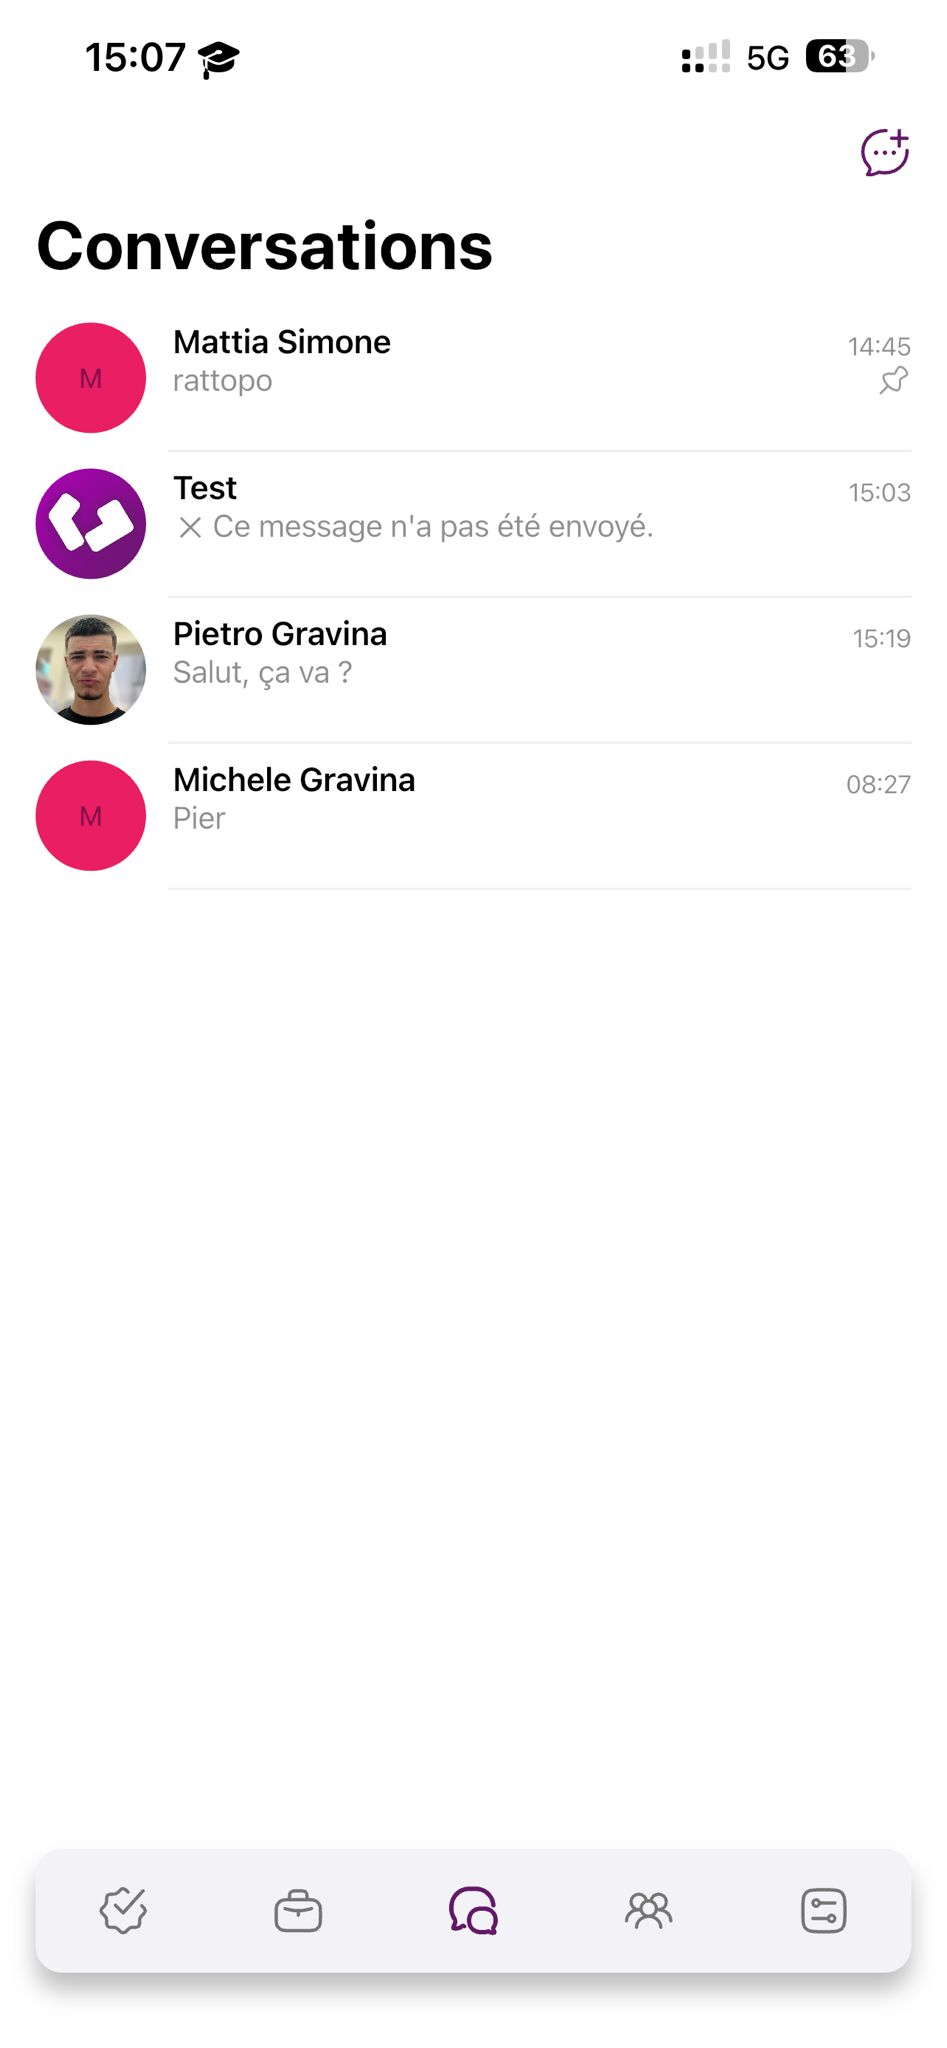
\includegraphics[width=\textwidth]{img/screenshots/chats_page.jpeg}}
			\caption*{\textbf{Liste des conversations} : affichage des contacts et des derniers messages reçus.}
		\end{minipage}
		\hfill
		\begin{minipage}[t]{0.45\textwidth}
			\centering
			\fbox{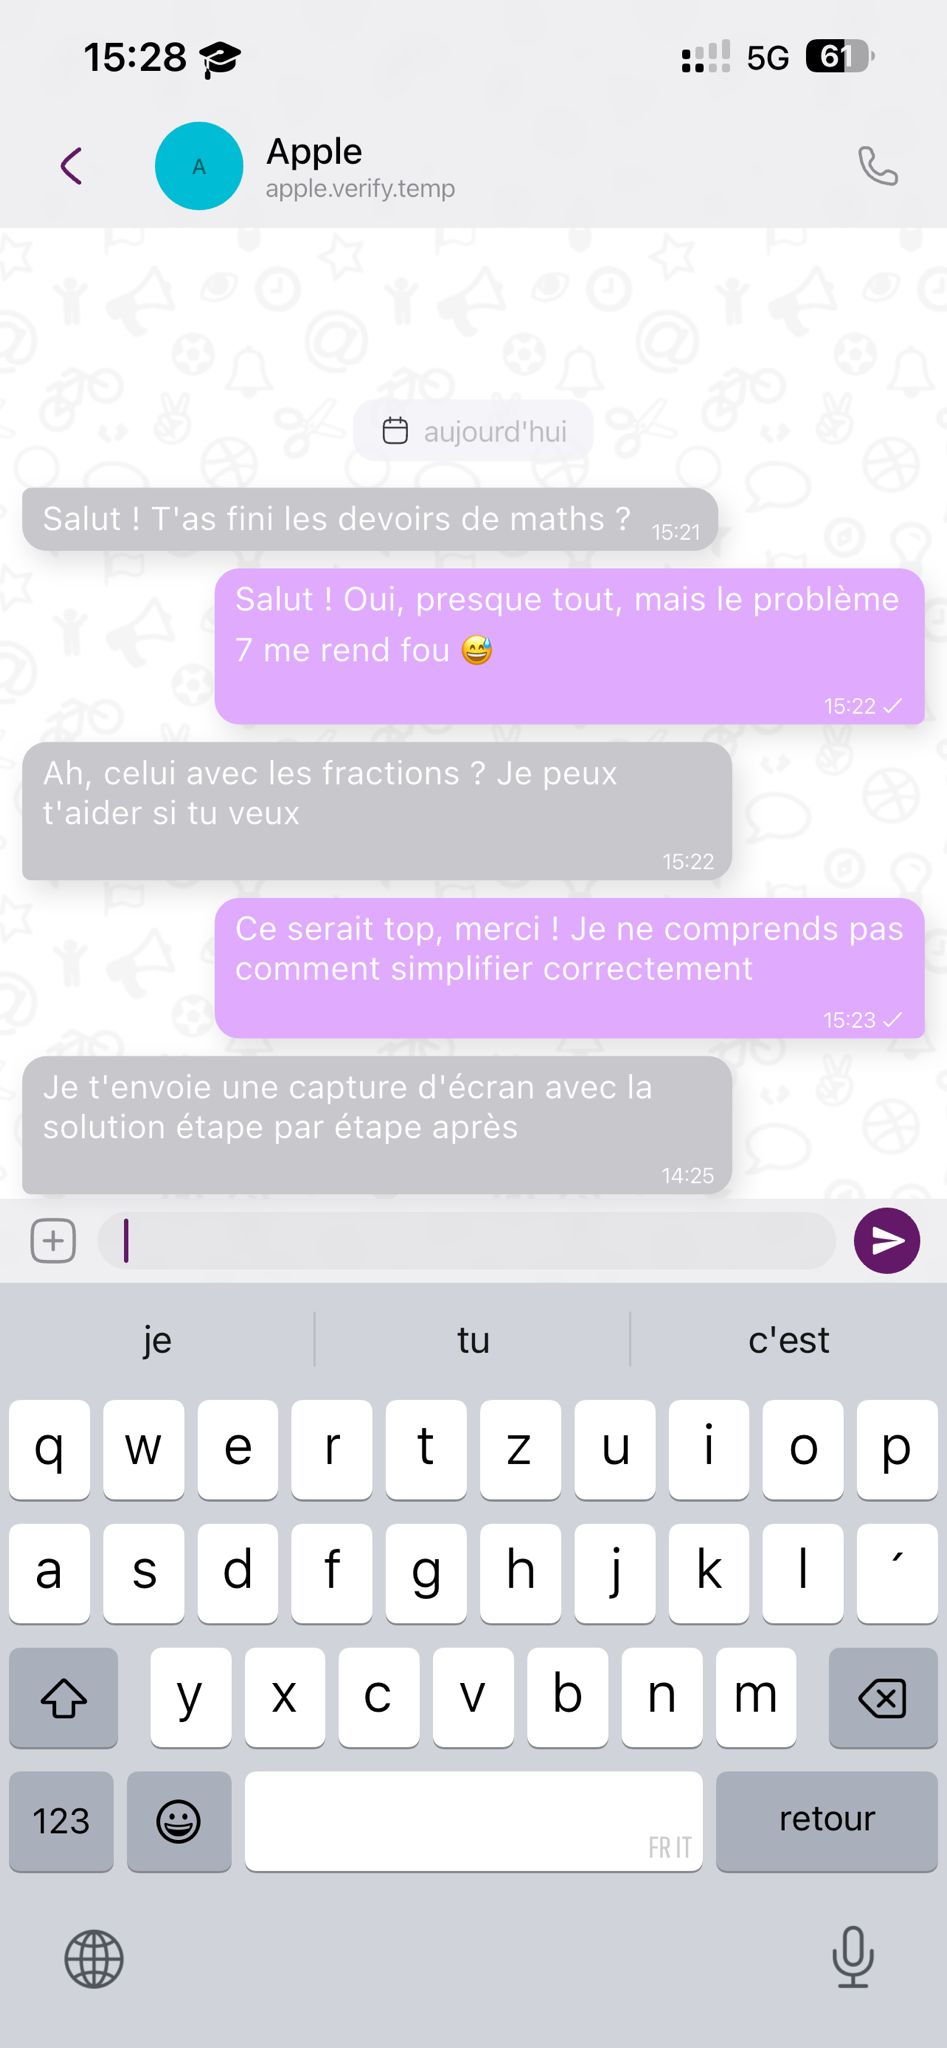
\includegraphics[width=\textwidth]{img/screenshots/chat_page.jpeg}}
			\caption*{\textbf{Fenêtre de discussion} : interface avec les messages envoyés et reçus.}
		\end{minipage}
	\end{figure}
	
	\begin{figure}[H]
		\centering
		\begin{minipage}[t]{0.45\textwidth}
			\centering
			\fbox{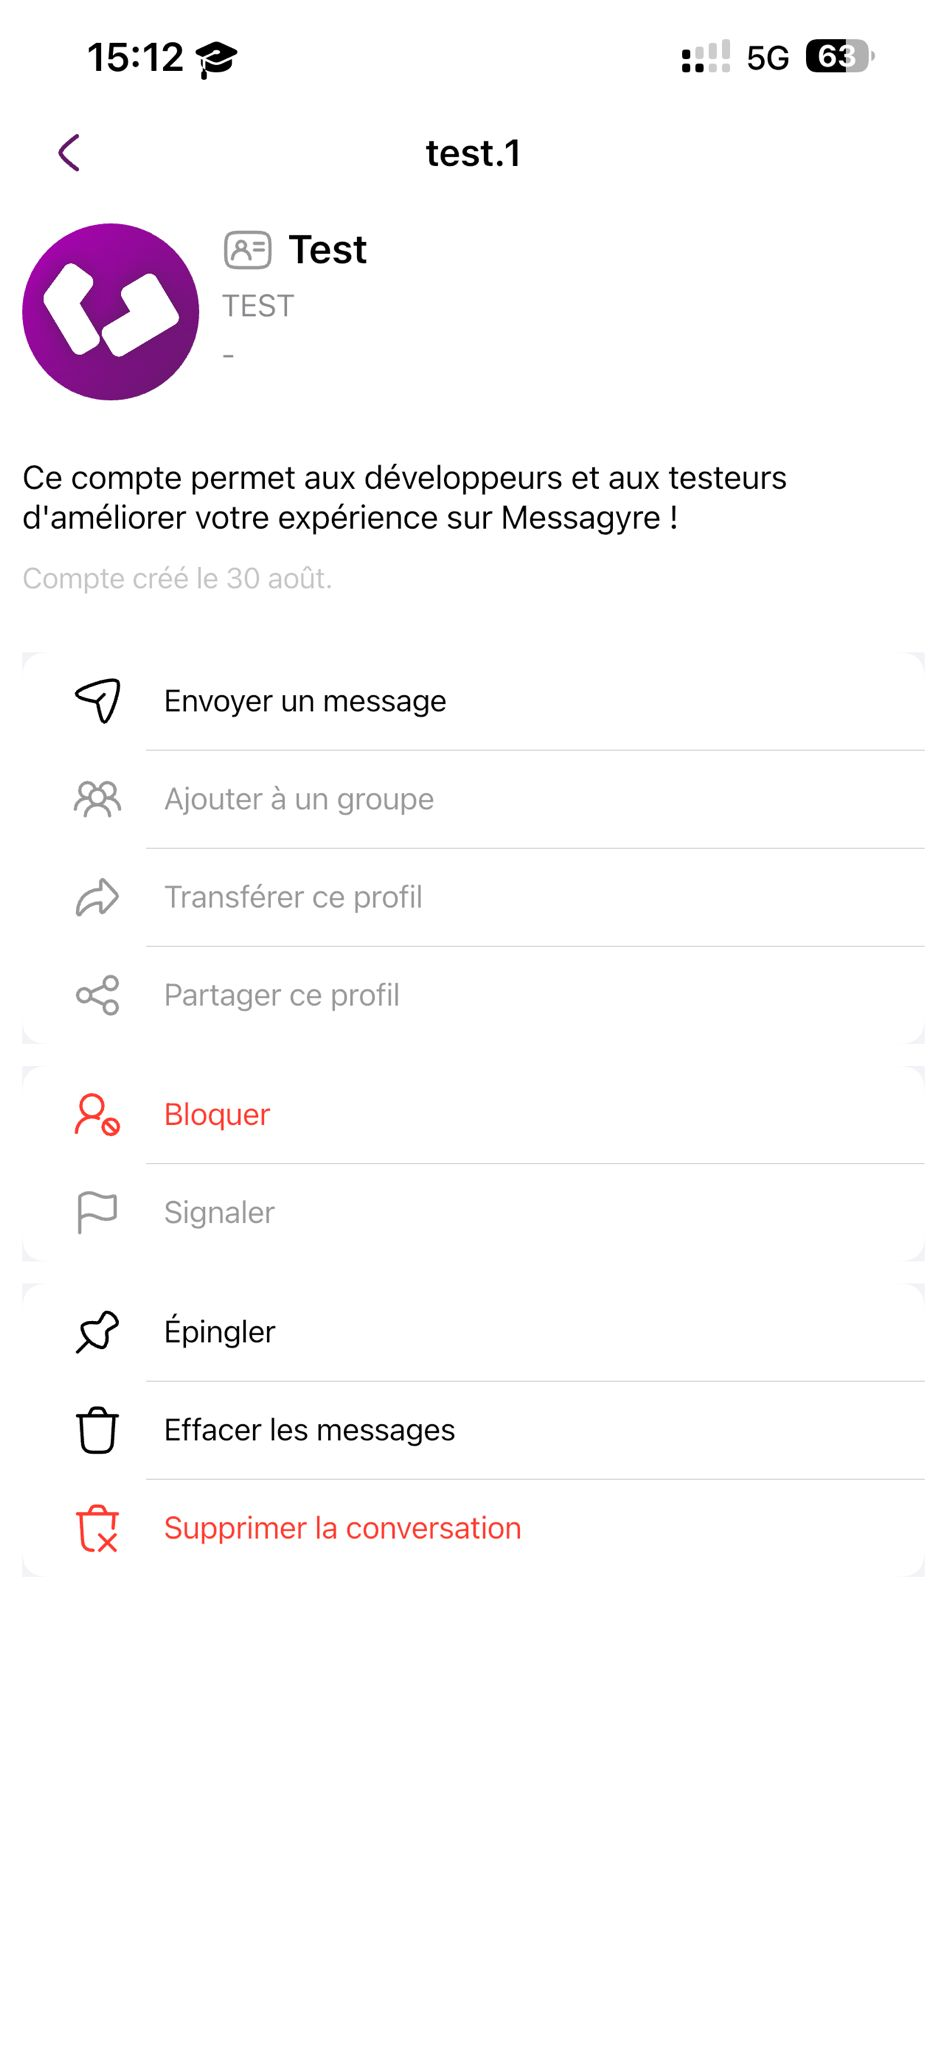
\includegraphics[width=\textwidth]{img/screenshots/profile_page.jpeg}}
			\caption*{\textbf{Profil utilisateur} : aperçu d’un compte avec photo et informations visibles.}
		\end{minipage}
	\end{figure}
	
	\begin{figure}[H]
		\centering
		\begin{minipage}[t]{0.45\textwidth}
			\centering
			\fbox{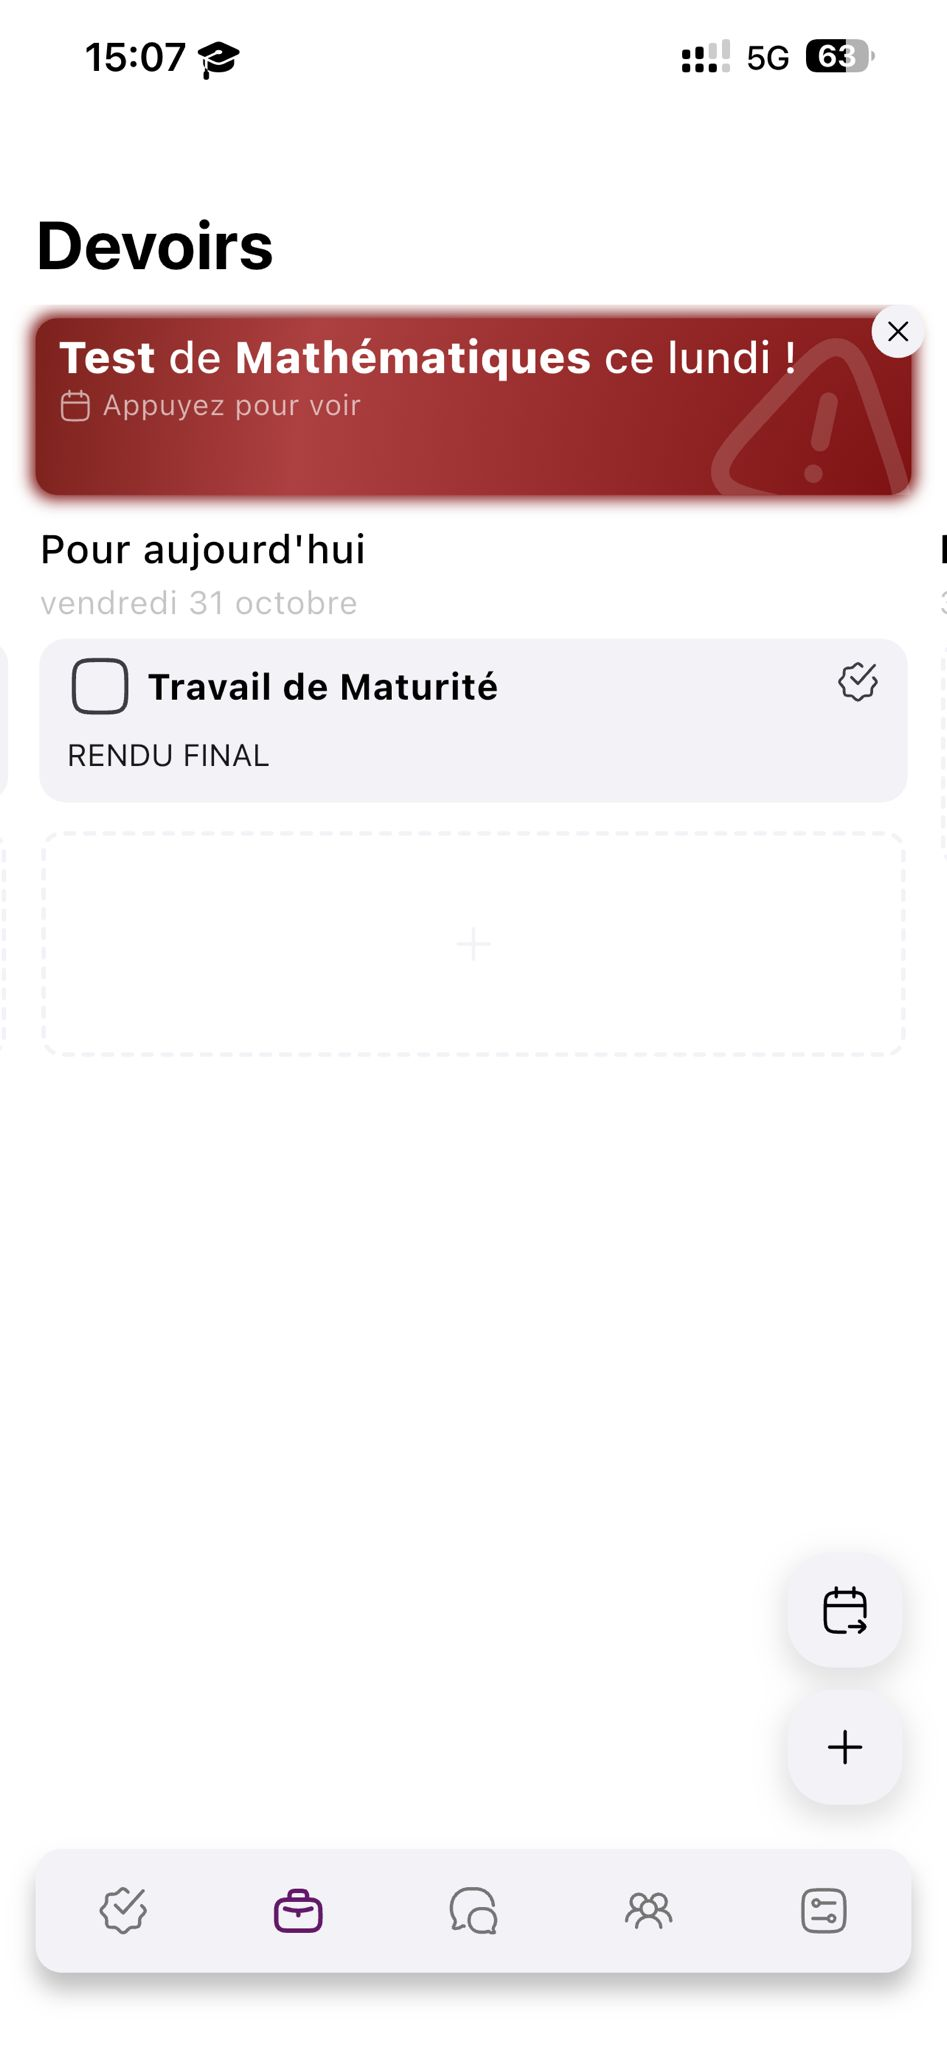
\includegraphics[width=\textwidth]{img/screenshots/homework_page.jpeg}}
			\caption*{\textbf{Page des devoirs} : liste des prochains devoirs, ajout d’un nouveau et visualisation des détails.}
		\end{minipage}
		\hfill
		\begin{minipage}[t]{0.45\textwidth}
			\centering
			\fbox{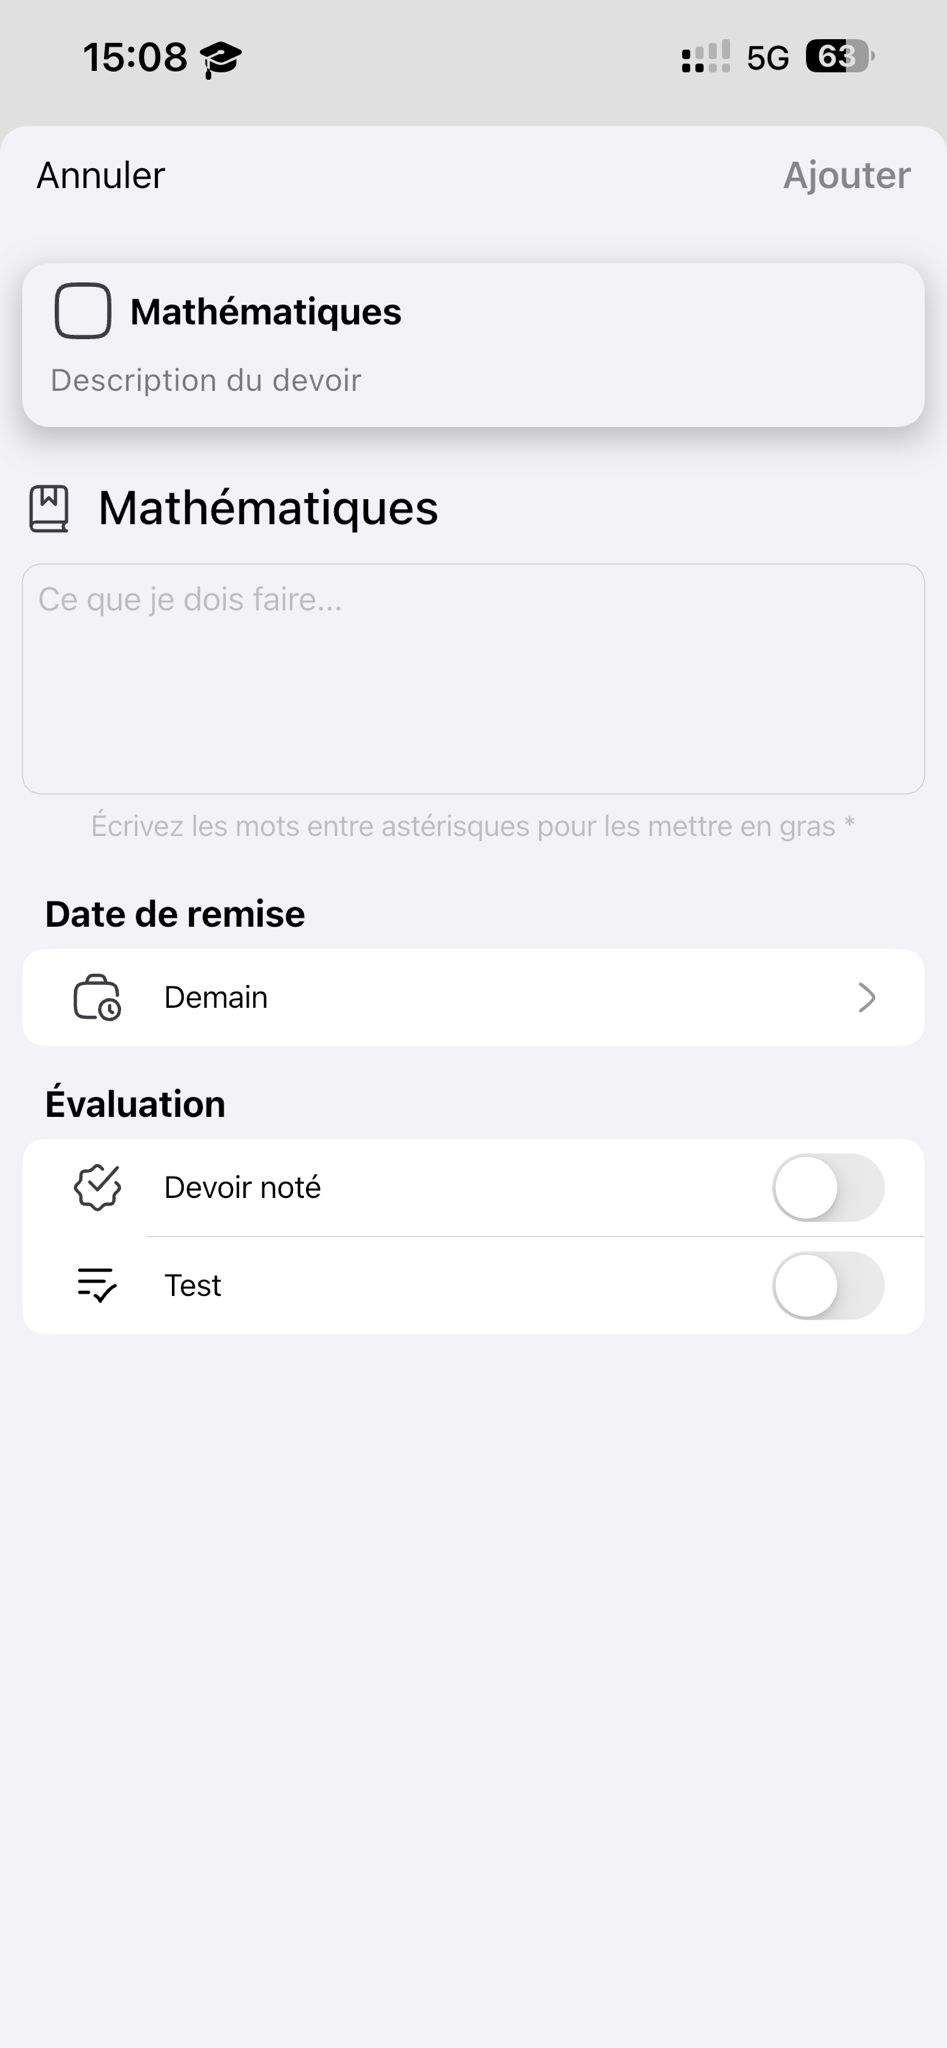
\includegraphics[width=\textwidth]{img/screenshots/add_homework_page.jpeg}}
			\caption*{\textbf{Ajout d'un devoir} : page qui permet à l'utilisateur d'ajouter un devoir à la liste.}
		\end{minipage}
	\end{figure}
	
	\begin{figure}[H]
		\centering
		\begin{minipage}[t]{0.45\textwidth}
			\centering
			\fbox{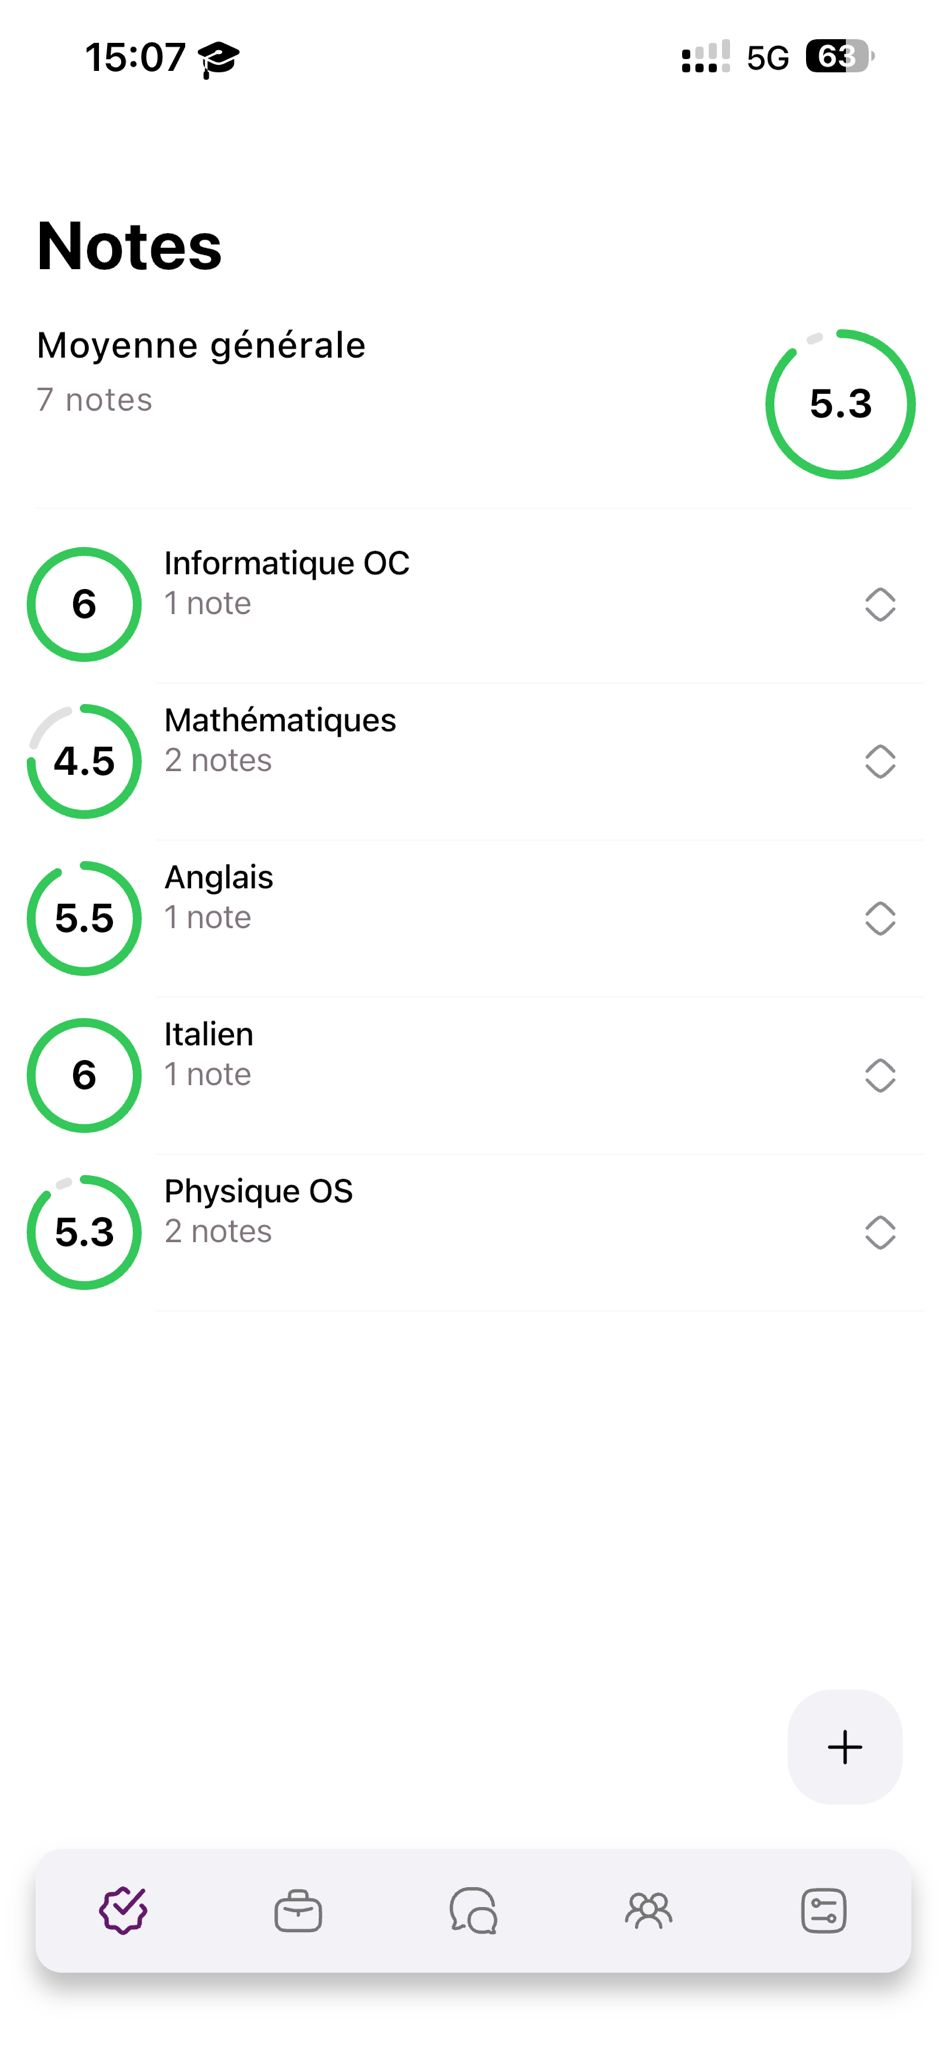
\includegraphics[width=\textwidth]{img/screenshots/grades_page.jpeg}}
			\caption*{\textbf{Page des notes} : affichage des moyennes et des résultats obtenus dans chaque matière.}
		\end{minipage}
		\hfill
		\begin{minipage}[t]{0.45\textwidth}
			\centering
			\fbox{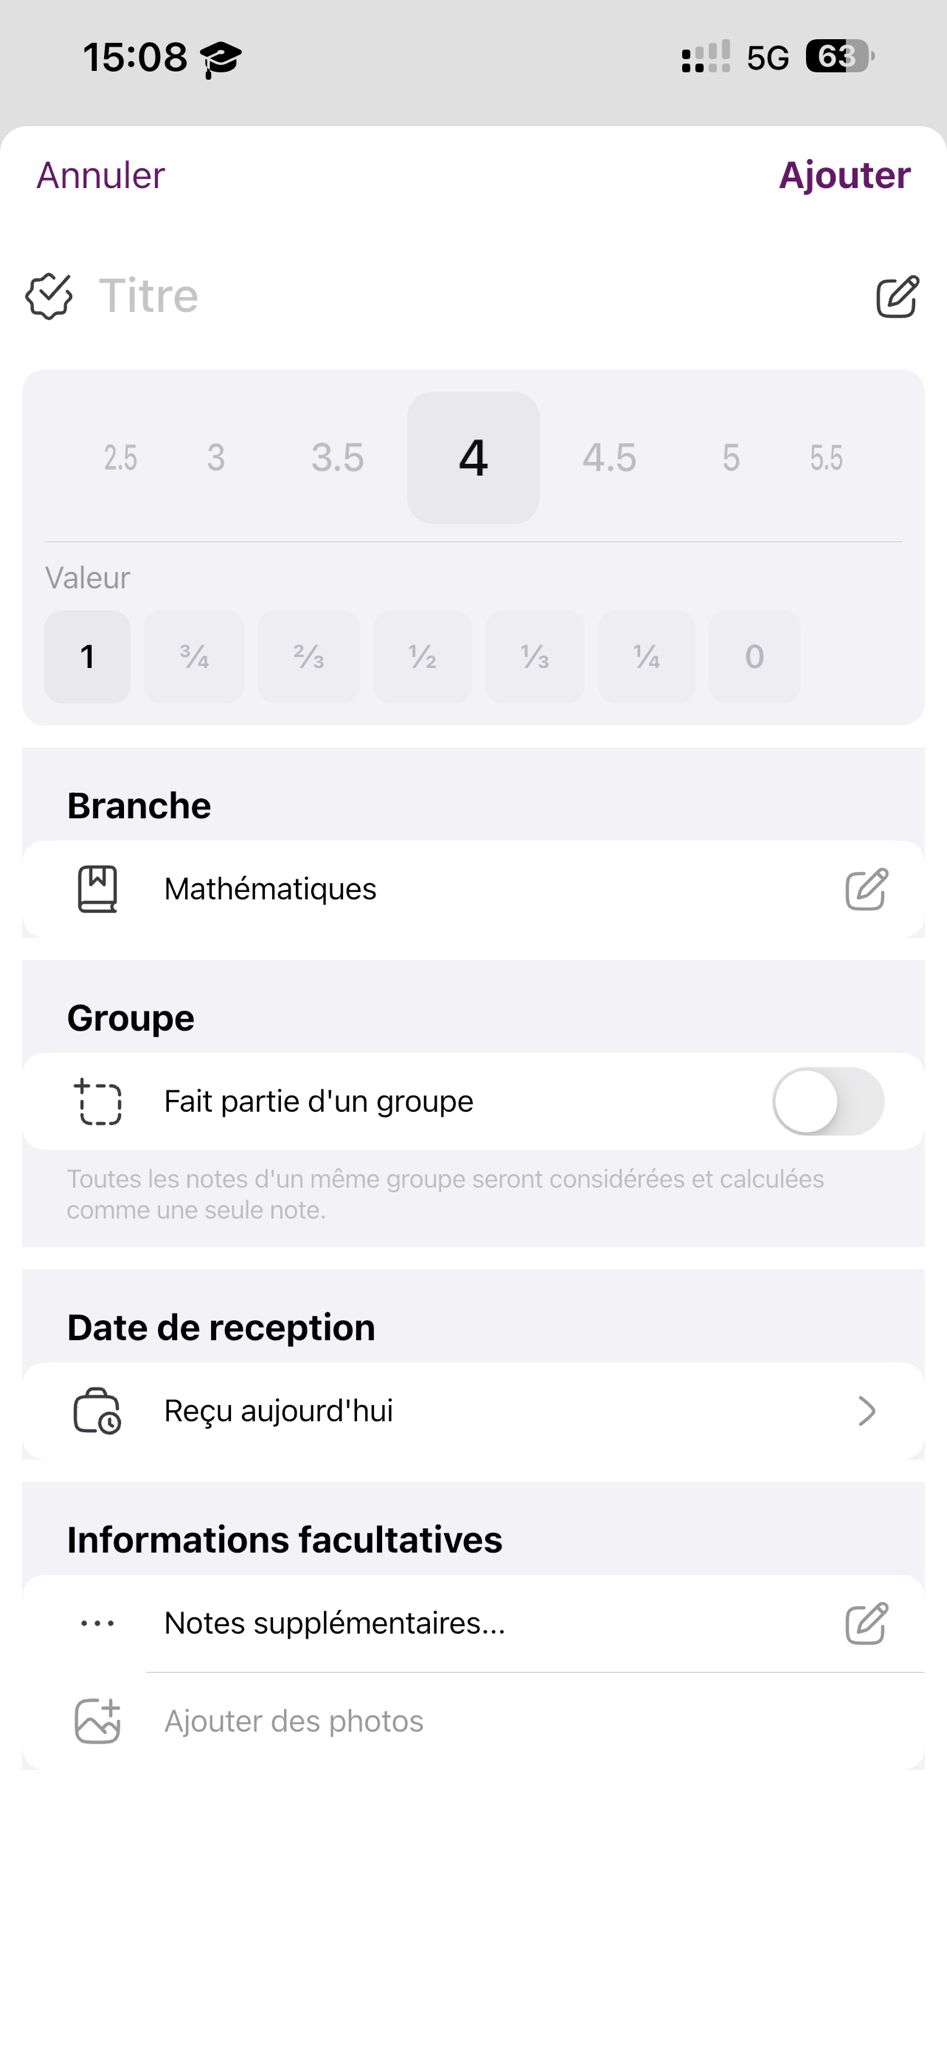
\includegraphics[width=\textwidth]{img/screenshots/add_grade_page.jpeg}}
			\caption*{\textbf{Ajout d’une note} : formulaire permettant d’ajouter une nouvelle note avec matière et coefficient.}
		\end{minipage}
	\end{figure}
	
	\begin{figure}[H]
		\centering
		\begin{minipage}[t]{0.45\textwidth}
			\centering
			\fbox{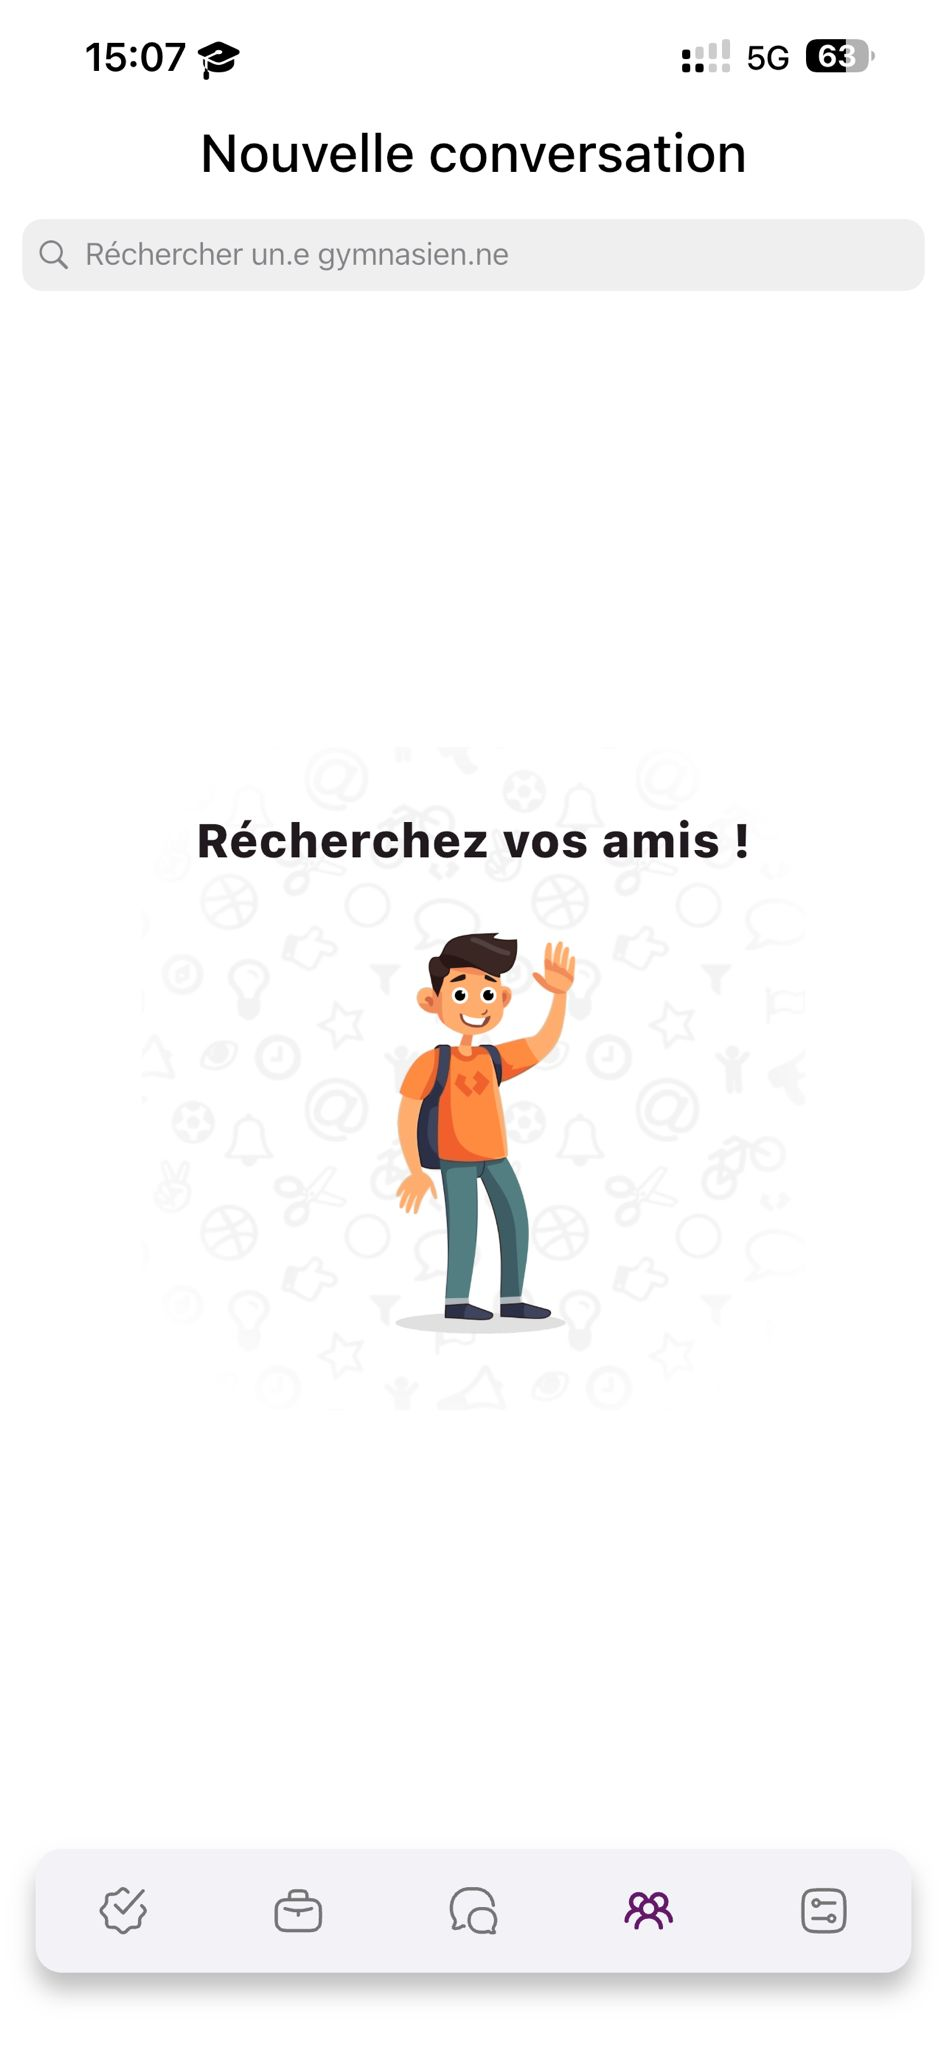
\includegraphics[width=\textwidth]{img/screenshots/search_page.jpeg}}
			\caption*{\textbf{Page de recherche} : permet de trouver d’autres utilisateurs ou conversations rapidement.}
		\end{minipage}
		\hfill
		\begin{minipage}[t]{0.45\textwidth}
			\centering
			\fbox{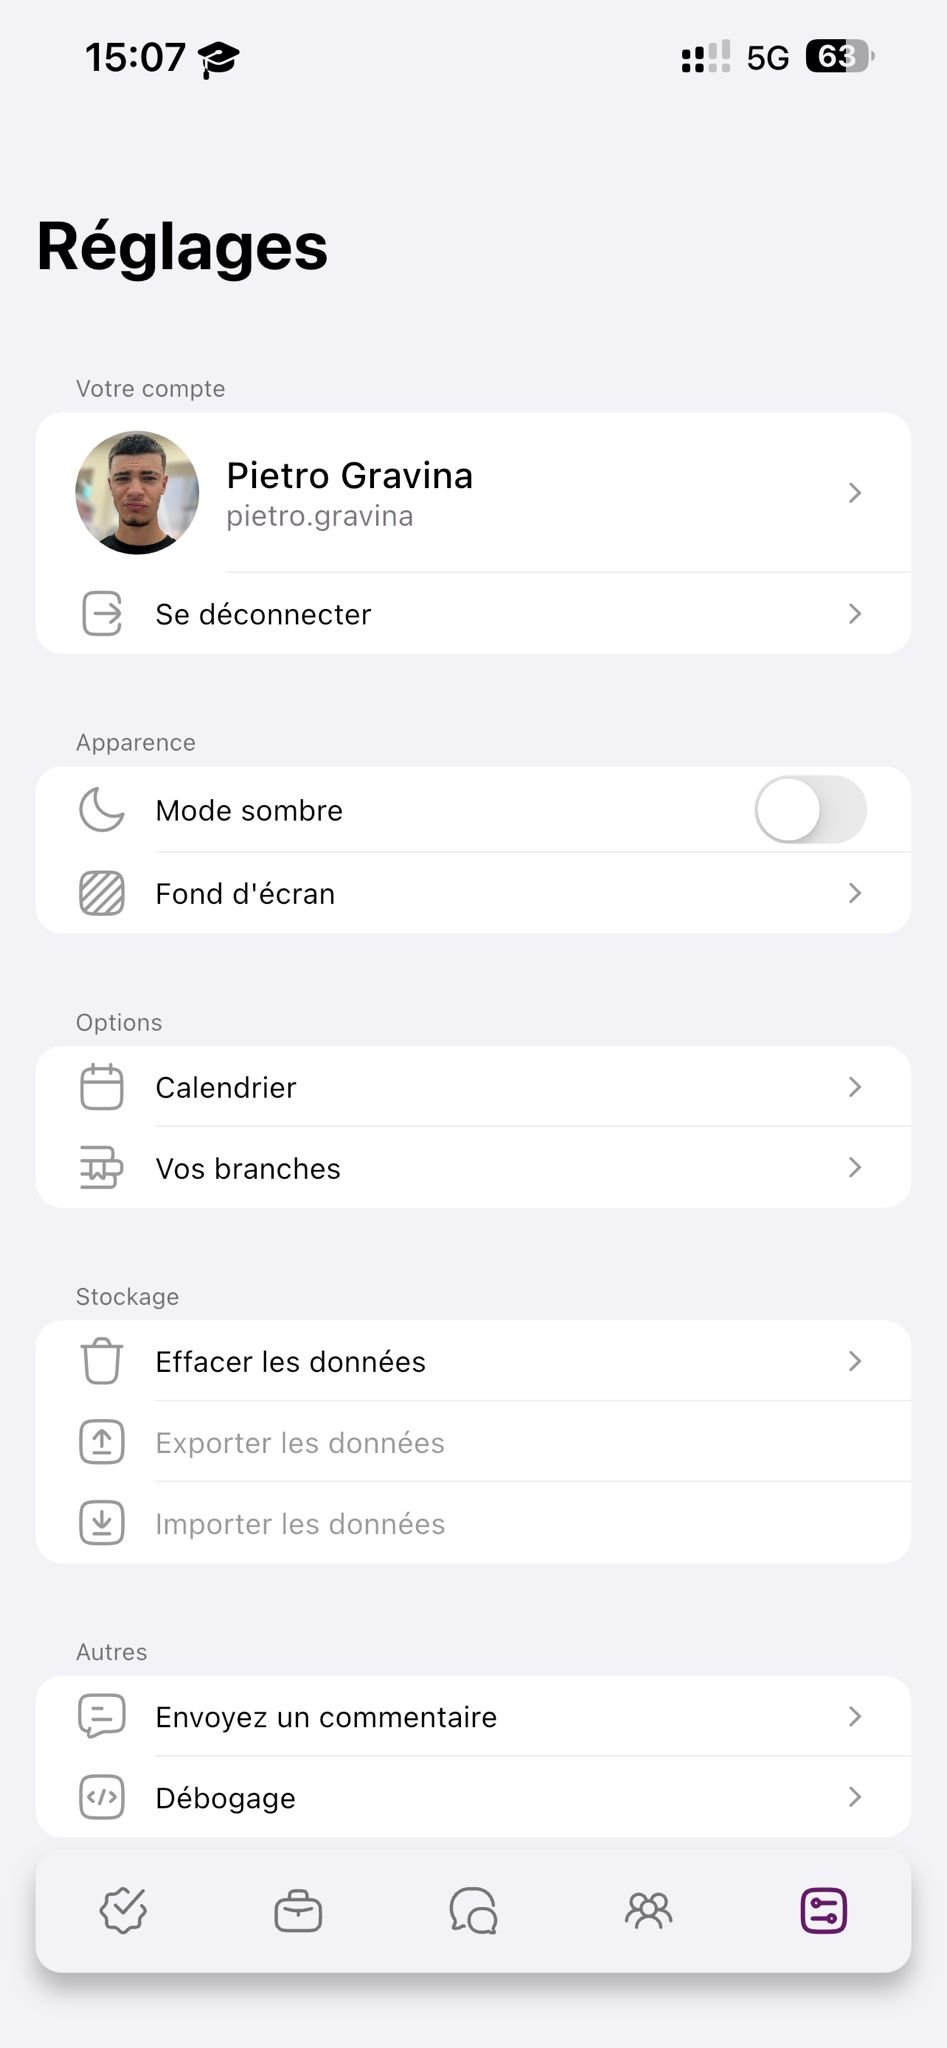
\includegraphics[width=\textwidth]{img/screenshots/settings_page.jpeg}}
			\caption*{\textbf{Page des paramètres} : options de personnalisation du profil et de gestion de l’application.}
		\end{minipage}
	\end{figure}
	
			
	\chapter{Difficultés rencontrées}
	
	\section{Difficultés techniques}
	
	Pendant le développement de Messagyre, j’ai dû faire face à de nombreuses difficultés techniques qui ont mis à l’épreuve mes connaissances et ma capacité d’adaptation.
	
	L’une des premières étapes du projet a été l’utilisation d’Unity comme client. Ce choix initial s’est vite révélé peu adapté au développement d’une application mobile. L’interface utilisateur était plus complexe à construire et les intégrations avec HTTP et WebSocket étaient laborieuses. Chaque élément devait être programmé manuellement : animations, dimensions, positionnement des composants, logique dynamique et visuelle. Tout devait être écrit depuis zéro, sans composants natifs adaptés aux appareils mobiles. Cette gestion artisanale prenait environ 90\% du temps de développement, ralentissant considérablement l’avancement du projet et rendant chaque modification fastidieuse. Le manque d’outils natifs pour les appareils mobiles a nui à l’expérience utilisateur, ce qui m’a poussé à migrer vers Flutter, bien plus adapté à une application moderne et fluide.
	
	Flutter a également posé des difficultés, notamment au début. N’ayant jamais utilisé ce framework auparavant, j’ai eu du mal à comprendre le cycle de vie des widgets et la gestion de l’état. L’intégration de paquets externes pour le chargement d’images, les animations et les notifications m’a demandé de nombreuses tentatives et beaucoup de débogage.
	
	L’un des défis les plus complexes a été la gestion de la communication en temps réel via WebSocket. En plus de devoir comprendre les différences avec HTTP, j’ai appris à gérer des connexions persistantes, des déconnexions inattendues et la synchronisation des messages entre le client et le serveur, tout en garantissant une bonne expérience utilisateur.
	
	La mise en place d’un système d’authentification sécurisé basé sur JWT et RefreshToken a également été une nouveauté pour moi. J’ai étudié des aspects liés à la cryptographie et à la sécurité des données pour assurer la fiabilité des sessions utilisateur. Le volet base de données n’a pas été plus simple : j’ai dû apprendre à configurer et utiliser MySQL, concevoir des tables avec des clés étrangères, optimiser les requêtes et gérer les erreurs de connexion, ce qui a demandé beaucoup de rigueur et de patience.
	
	Le déploiement sur Railway m’a aussi posé des problèmes de compatibilité entre différentes versions de .NET. Adapter le projet à une version stable supportée, sans perdre en performance, a été un défi supplémentaire.
	
	\section{Hébergement et budget}
	\label{hostingandbudget}
	
	Une difficulté importante a été de trouver une plateforme en ligne, un service externe, pour héberger le serveur ASP.NET Core. En effet, exécuter le programme que j’ai écrit pour le serveur de Messagyre nécessite certaines caractéristiques qui ne sont pas facilement accessibles, comme une adresse IP statique, indispensable pour être toujours visible par les appareils du monde entier et leur permettre de se connecter. Je cherchais une solution compatible avec la technologie .NET, mais aussi la plus économique possible, n’ayant pas une grande disponibilité financière. Après plusieurs recherches et essais, j’ai d’abord opté pour \textbf{Railway}, une plateforme moderne, facile à configurer et dotée d’une immense communauté, offrant un support complet et réactif.
	
	Cependant, le coût initial était trop élevé pour moi : environ 3 francs par jour selon les estimations, ce qui représentait une dépense difficilement soutenable à long terme. J’avais envisagé de demander un financement à l’école, mais dans le contexte actuel, il est déjà difficile d’obtenir des fonds pour du matériel scolaire classique, alors un hébergement web non réutilisable paraissait encore moins justifiable.
	
	J’ai donc décidé de calculer les dépenses annuelles et de chercher des alternatives. La solution retenue a été de passer à un \textbf{modèle serverless}, également proposé par Railway, qui permet un hébergement gratuit pendant la phase de développement, puis un forfait d’environ 5 francs par mois au moment de la publication. Ce compromis m’a permis de poursuivre le projet sans frais.
	
	Plus tard, je me suis rendu compte que le plan gratuit de cette plateforme était trop limité, bloquant tout après quelques utilisations par mois. Cela m’a conduit à chercher une autre plateforme, et j’ai trouvé \textbf{Fly.io}.
	
	Par rapport à Railway, celle-ci est beaucoup moins une « boîte noire », me permettant de mieux configurer l’environnement, mais elle a présenté certains problèmes que je n’avais pas auparavant, comme le blocage des serveurs SMTP : un service que j’utilisais pour envoyer les e-mails de vérification aux nouveaux utilisateurs. J’ai donc dû passer par les API de Google, ce qui m’a offert moins de liberté de configuration.
	
	Quelques mois après être passé sur cette nouvelle plateforme, je me suis rendu compte que j’utilisais beaucoup trop de services tiers : un pour stocker les photos de profil des utilisateurs, un pour envoyer les e-mails de vérification, un autre pour la base de données des utilisateurs, et ainsi de suite. Bien que l’application puisse fonctionner parfaitement avec tous ces services, le développement devenait plus complexe. Chacun de ces services proposait un plan gratuit limité, au-delà duquel il fallait souscrire à un abonnement mensuel ; additionnés, ces coûts auraient dépassé largement mon budget.
	
	J’ai discuté de ce problème avec mon professeur d’Option Complémentaire d’Informatique, Micha Hersch, qui m’a gentiment proposé d’utiliser l’un de ses serveurs, qu’il employait déjà pour partager du matériel avec la classe d’OC — une proposition que je ne pouvais refuser, puisqu’elle résolvait bon nombre des problèmes rencontrés jusque-là. Je me suis donc organisé avec lui, j’ai modifié le programme et je l’ai transféré sur son serveur. Grâce à ce passage très rapide, les problèmes comme la lenteur d’accès à l’application, les serveurs qui ne répondaient pas, les déconnexions après peu de temps d’utilisation, et surtout le temps exagéré nécessaire pour appliquer des modifications au code du serveur, ont été résolus.
	
	Actuellement, même si le professeur m’a permis d’utiliser son serveur jusqu’à la fin de l’année scolaire, ce changement me permet de ne supporter aucun coût pour faire fonctionner l’application, ce qui m’a permis — et me permettra encore — de continuer à développer le projet sans limites et sans devoir passer des heures à chercher le moyen le moins coûteux d’ajouter de nouvelles fonctionnalités à l’application.
	
	\section{Difficultés organisationnelles}
	
	Outre les aspects techniques, j’ai rencontré des difficultés organisationnelles. Réussir à concilier le développement du projet avec les cours, les devoirs et la vie personnelle n’a pas été simple. J’ai dû apprendre à mieux gérer mon temps, établir des plannings réalistes et éviter la procrastination.
	
	Parfois, la motivation diminuait, surtout dans les moments où les résultats tardaient ou lorsque les problèmes semblaient insurmontables. Mais voir l’application fonctionner concrètement sur le téléphone de mes amis m’a redonné de l’énergie pour continuer.
	
	\section{Comment j’ai surmonté les difficultés}
	
	Pour surmonter ces obstacles techniques et organisationnels, je me suis appuyé principalement sur l’apprentissage autodidacte, avec l’aide précieuse des intelligences artificielles. J’ai consulté la documentation officielle, suivi des tutoriels, lu des discussions sur des forums comme Stack Overflow et GitHub, et expérimenté différentes approches jusqu’à trouver les bonnes solutions.
	
	Les intelligences artificielles se sont révélées être des outils extrêmement efficaces : elles m’ont souvent proposé des solutions optimisées, ce qui m’a fait gagner un temps précieux. Elles m’ont aussi permis d’écrire du code plus propre et de découvrir des bibliothèques ou des paquets que je n’aurais probablement jamais trouvés seul, accélérant ainsi significativement le développement.
	
	J’ai appris à diviser mon travail en objectifs concrets et atteignables, ce qui m’a permis de progresser étape par étape sans me décourager. Parler du projet avec des amis ou des enseignants m’a également aidé à clarifier mes idées et à trouver de nouvelles pistes.
	
	Toutes ces expériences, bien que parfois éprouvantes, m’ont permis de grandir, aussi bien techniquement que dans la gestion de projet et l’autonomie.
	
	
	\chapter{Bilan personnel}
	
	Ce projet m’a permis de vivre une expérience de développement complète, avec toutes les phases que cela implique : conception, recherche, programmation, tests, déploiement et documentation. Sur le plan technique, j’ai énormément appris. J’ai approfondi mes compétences en C\#, découvert ASP.NET Core, compris en profondeur le fonctionnement des WebSocket et de l’authentification via JWT. J’ai également acquis une grande maîtrise de Flutter et du développement mobile multiplateforme, ainsi que des bases de données MySQL.
	
	Sur le plan personnel, ce travail m’a appris la persévérance, la rigueur et l’autonomie. J’ai dû me former seul sur de nombreuses technologies complexes, souvent sans aide extérieure directe. J’ai aussi pris conscience de l’importance de bien planifier son temps et de savoir demander de l’aide au bon moment. Ce projet m’a donné confiance en ma capacité à mener une idée de bout en bout, même face à des obstacles importants.
	
	Si je devais refaire ce projet, je choisirais dès le départ des outils plus adaptés aux besoins d’une application mobile. J’éviterais Unity, dont la flexibilité est un atout dans le domaine du jeu vidéo, mais un inconvénient majeur dans ce type d’application. J’organiserais aussi mieux mon temps dès le début, avec une feuille de route plus précise et un système de gestion des tâches plus rigoureux.
	
	Quant à l’avenir de Messagyre, je n’exclus pas de continuer à le développer et à l’améliorer. Plusieurs idées restent à concrétiser, comme l’ajout de notifications push, une version web de l’application, l’intégration de messages vocaux ou vidéos, ou encore une meilleure gestion des groupes et des discussions collectives. Le projet pourrait même, un jour, être proposé à d’autres écoles, au-delà du Gymnase de Renens, si son usage s’y prête.
	
	En somme, cette expérience a été à la fois un défi technique et une aventure personnelle très enrichissante, qui m’a beaucoup apporté et dont je suis fier.
	
	
	\chapter{Conclusion}
	
	Le développement de Messagyre a représenté pour moi un parcours long, exigeant et formateur. De l’idée initiale à la réalisation de l’application, j’ai traversé de nombreuses étapes : changements de technologies, obstacles techniques, réécritures complètes et améliorations successives. Chaque choix, même ceux qui semblaient initialement erronés, a contribué à construire un projet solide et concret.
	
	D’un point de vue technique, j’ai pu expérimenter de manière pratique de nombreuses compétences acquises au fil des années, en consolider de nouvelles et approfondir des technologies complexes comme Flutter, ASP.NET Core, JWT et WebSocket. Mais au-delà des aspects techniques, j’ai acquis une méthode de travail plus organisée et plus consciente, en affrontant des problèmes réels et en apprenant à chercher des solutions efficaces.
	
	Messagyre n’est pas seulement une application de messagerie : c’est le résultat de centaines d’heures de travail, d’essais, d’erreurs et de corrections. C’est aussi la preuve qu’un projet ambitieux peut devenir réalité, même s’il est développé par une seule personne, avec passion et détermination.
	
	Personnellement, je considère ce projet comme l’un des travaux les plus complets et significatifs que j’aie jamais réalisés. Il a une grande valeur, tant du point de vue professionnel — car il démontre mes compétences de développeur — que du point de vue personnel — car il m’a appris à croire en mes idées et à les porter jusqu’au bout avec détermination.
	
	J’espère que Messagyre pourra continuer à évoluer au-delà de ce travail de maturité. Qu’il puisse être utile aux élèves et aux enseignants, et peut-être devenir un véritable outil de communication scolaire, simple, sécurisé et accessible à tous.
	
	\chapter{Annexes}
	
	\section{Code source}
	
	Le code complet du projet est disponible sur GitHub aux adresses suivantes :
	
	\begin{itemize}
		\item \textbf{Client Flutter} : \url{https://github.com/Gravi32/MessagyreClient}
		\item \textbf{Serveur ASP.NET Core} : \url{https://github.com/Gravi32/MessagyreServer}
	\end{itemize}
	
	Pour faciliter l’accès, voici deux codes QR menant aux dépôts.
	
	\begin{figure}[H]
		\centering
		\begin{minipage}[t]{0.32\textwidth}
			\centering
			\fbox{
\includegraphics[width=\textwidth]{img/client_repo_qr_code.png}}
			\caption*{Dépôt GitHub du Client}
		\end{minipage}
		\hfill
		\begin{minipage}[t]{0.32\textwidth}
			\centering
			\fbox{
\includegraphics[width=\textwidth]{img/server_repo_qr_code.png}}
			\caption*{Dépôt GitHub du Serveur}
		\end{minipage}
		
	\end{figure}
	
	\section{Diagrammes}
	\label{diagrams}
	
	Pour illustrer la structure et l’architecture du projet, un diagramme UML expliquant le fonctionnement du backend de l'application a été réalisé et est disponible au lien suivant :
	
	\url{https://lucid.app/lucidchart/b8dadd52-61fd-468b-8bd6-a81aa133eb02/edit?viewport_loc=-3637\%2C-1769\%2C9681\%2C4831\%2C0_0&invitationId=inv_fa22bca5-082d-4666-b827-15f4adaa3a38}
	
	\begin{figure}[H]
		\centering
		\begin{minipage}[t]{0.32\textwidth}
			\centering
			\fbox{
\includegraphics[width=\textwidth]{img/server_uml_qr_code.png}}
			\caption*{Diagramme UML du backend}
		\end{minipage}
		\hfill
		
		
	\end{figure}
	
	
	\section{Icônes de l’application}
	
	Voici les icônes de l'application utilisées dans Messagyre pendant la premiere partie du développement :
	
	\begin{figure}[H]
		\centering
		\begin{minipage}[t]{0.45\textwidth}
			\centering
			
\includegraphics[width=0.7\textwidth]{img/logo_purple.png}
			\caption{Icône violette (version simplifiée)}
		\end{minipage}
		\hfill
		\begin{minipage}[t]{0.45\textwidth}
			\centering
			
\includegraphics[width=0.7\textwidth]{img/logo_full.png}
			\caption{Icône complète de l’application}
		\end{minipage}
	\end{figure}
	
	Après quelques mois, j’ai décidé de modifier cette icône afin d’obtenir un rendu plus moderne, esthétique et cohérent avec le style des applications contemporaines. Voici trois versions de la même icône, réalisées pour différents cas d’utilisation :
	
	
	\begin{figure}[H]
		\centering
		\begin{minipage}[t]{0.32\textwidth}
			\centering
			
\includegraphics[width=0.7\textwidth]{img/rounded_logo_purple.png}
			\caption{Icône violette arrondie pour fonds clairs}
		\end{minipage}
		\hfill
		\begin{minipage}[t]{0.32\textwidth}
			\centering
			
\includegraphics[width=0.7\textwidth]{img/rounded_logo_white.png}
			\caption{Icône blanche arrondie pour fonds sombres}
		\end{minipage}\hfill
		\begin{minipage}[t]{0.32\textwidth}
			\centering
			
\includegraphics[width=0.7\textwidth]{img/rounded_logo_full.png}
			\caption{Icône arrondie complète de l’application}
		\end{minipage}
	\end{figure}
	
	J’ai choisi la couleur principale de l’application, la nuance de violet présente dans toutes les icônes ainsi que dans plusieurs éléments de l’interface, en m’inspirant de la couleur du logo officiel du Gymnase de Renens :
	
	\begin{figure}[H]
		\centering
		\begin{minipage}[t]{0.32\textwidth}
			\centering
			
\includegraphics[width=0.7\textwidth]{img/logo_gyre.png}
			\caption{Logo officiel du Gymnase de Renens}
			\url{https://www.gyre.ch}
		\end{minipage}
		\hfill
		
	\end{figure}
	
	\section{Structure du serveur}
	
	Chaque composant du serveur est expliqué dans les sous-sections à venir, qui présenteront un \textit{"Extrait du code"}, c’est-à-dire une illustration schématique du code du composant. Il est possible de visiter le \href{https://github.com/Gravi32/MessagyreServer.git}{dépôt GitHub} du projet du serveur pour accéder au code complet.
	Pour comprendre plus facilement le fonctionnement des différents composants du serveur, un \href{https://lucid.app/lucidchart/b8dadd52-61fd-468b-8bd6-a81aa133eb02/edit?viewport_loc=-3637\%2C-1769\%2C9681\%2C4831\%2C0_0&invitationId=inv_fa22bca5-082d-4666-b827-15f4adaa3a38}{Diagramme UML} (voir la section Diagrammes \ref{diagrams}) est également disponible.
	
	\begin{center}
		\textbf{\textcolor{red}{Attention :}} Cette section a été la première rédigée pour ce travail. Le code présenté n’est donc \textbf{ni complet ni entièrement à jour}.
	\end{center}
	
	\subsection{User.cs}
	
	Lorsqu’un serveur reçoit une requête, il est souvent nécessaire de pouvoir reconnaître, distinguer et cataloguer l’expéditeur : cela est représenté par la classe \code{User}, une classe non statique (donc instanciable) contenant toutes les informations utiles concernant l’utilisateur connecté.
	
	\subsubsection{Extrait du code}
	\begin{minted}{csharp}
using System.Net.WebSockets;

namespace MessagyreServer.Classes
{
	public class User
	{
		public Account? Account { get; private set; }
		public WebSocket Socket { get; }
		public bool IsAuthorized { get; private set; }
		public string RegistrationEmailAddress = "";
		public string RegistrationTempEmailAddress = "";
		public int RegistrationVerificationCode;
		public DateTime RegistrationCodeSentAt;
		
		public User(WebSocket Socket)
		{
			this.Socket = Socket;
		}
		
		public void Receive(Signal SignalToSend)
		{
			Socket.Send(SignalToSend.Pack());
		}
		
		public void Authenticate(Account? GivenAccount)
		{
			Account = GivenAccount;
			IsAuthorized = GivenAccount != null;
		}
	}
}
	\end{minted}
	
	\subsubsection{Variables principales}
	Une instance de la classe \code{User} contient trois informations principales : le compte (\code{Account}) lié à l'utilisateur (si authentifié), le \code{Socket} du client connecté (nécessaire pour pouvoir lui envoyer des messages), et un booléen \code{IsAuthorized} qui indique si l'utilisateur s'est connecté à son compte ou non.
	
	\subsubsection{Methodes}
	Le premier "méthode" de ce script est un \code{Constructor}, il est appelé lorsque la classe est instanciée et stocke le \code{Socket} en mémoire.
	
	Le second est uniquement pour la lisibilité, lorsqu'il est appelé, il envoie le message \code{Signal} au client.
	
	Le dernier (\code{Authenticate()}), est appelé par la classe \code{Authenticator} lorsque l'utilisateur se connecte à son compte.
	\\\\
	
	\subsection{Signal.cs}
	
	Une autre classe non statique qui contient toutes les informations d'une requête/message. Elle est instanciée lorsque le serveur reçoit une requête ou lorsqu'il doit envoyer un message à un client spécifique.
	
	\subsubsection{Extrait du code}
	
	\begin{minted}{csharp}
using Newtonsoft.Json;

namespace MessagyreServer.Classes
{
	public class Signal
	{
		[JsonIgnore] public User? Sender;
		
		public SignalType Type;
		public Dictionary<string, string> Data = new();
		
		public Signal(SignalType Type, User? Sender = null)
		{
			this.Type = Type;
			this.Sender = Sender;
		}
		
		public string Pack()
		{
			return JsonConvert.SerializeObject(this);
		}
		
		public static Signal? Unpack(string Source, User Sender)
		{
			Signal? Result;
			
			try { 
				Result = JsonConvert.DeserializeObject<Signal>(Source); 
				}
			catch { return null; }
			
			if (Result != null) Result.Sender = Sender;
			
			return Result;
		}
		
	}
	
	public enum SignalType
	{
		Login, 
		Registration, 
		Logout,
		Message,
		Search
	}
}
	\end{minted}
	
	\subsubsection{Variables principales}
	Les informations contenues dans cette classe sont réparties en trois variables :
	
	1.\code{Sender} Indique l'utilisateur à partir duquel le serveur a reçu le message. 
	\code{[JsonIgnore]} indique au Serializer de Newtonsoft.Json que la variable ne doit pas être incluse dans le contenu du Json lorsque l'instance de la classe sera stockée en mémoire non volatile. (voir Messages.cs)
	
	2.\code{Type} Indique de quel type de \code{Signal} il s'agit, les options possibles se trouvent dans l’\code{enum} \code{SignalType} en bas du script.
	
	3.\code{Data} Contient un “dictionnaire” (une liste où chaque élément a un nom) avec toutes les données du \code{Signal}, par exemple \code{Username} et \code{Password} dans le cas d'un \code{Signal} de \code{Type} \code{SignalType.Login}.
	
	\subsubsection{Methodes}
	La méthode \code{Pack} “emballe” le \code{Signal}, c'est-à-dire qu'elle convertit les trois variables en un objet \textit{Json} via la méthode \code{SerializeObject} de \code{JsonConvert}, provenant de la bibliothèque \code{Newtonsoft.Json}. Cela est nécessaire pour pouvoir l'envoyer au client, car il n'est pas possible d'envoyer des instances de classes via \textit{WebSocket}, mais uniquement des chaînes de caractères.
	
	\code{Unpack} fait exactement l'inverse, en prenant une chaîne contenant l'objet \textit{Json}, elle la “convertit” en une nouvelle instance de \code{Signal}. Cette action est entourée d'un \code{try catch} car si un client devait envoyer une requête avec des données corrompues, mal formatées ou s'il y avait un problème lors de la transmission, le \textit{Json} ne serait pas valide et le serveur planterait.
	\\\\
	\subsection{Account.cs}
	Dernière classe non statique qui représente le compte d'un utilisateur.
	
	\subsubsection{Extrait du code}
	\begin{minted}{csharp}
using Newtonsoft.Json;

namespace MessagyreServer.Classes
{
	public class Account
	{
		public string Username { get; set; }
		public string Password { get; private set; }
		public string EmailAddress { get; set; }
		public DateTime CreationDate { get; }
		public DateTime? LastLogin { get; set; }
		public bool Banned { get; set; }
		
		public List<Signal> Inbox { get; set; } = new();
		
		
		// Constructors 
		public Account(
			string username, 
			string password, 
			string emailAddress)
		{
			Username = username;
			Password = Hash(password);
			EmailAddress = emailAddress;
			CreationDate = DateTime.UtcNow;
		}
		
		[JsonConstructor]
		public Account(
			string username, 
			string password, 
			string emailAddress, 
			DateTime creationDate, 
			DateTime? lastLogin,
			bool banned)
		{
			Username = username;
			Password = password;
			EmailAddress = emailAddress;
			CreationDate = creationDate;
			LastLogin = lastLogin;
			Banned = banned;
		}
		
		
		
		// Private methods 
		private static string Hash(string Password) 
			=> BCrypt.Net.BCrypt.HashPassword(Password);
		
		
		
		// Public methods 
		public bool TryPassword(string Attempt) 
			=> BCrypt.Net.BCrypt.Verify(Attempt, Password);
		
		public static string GetUsernameFromEmail(string Address) 
			=> Address.Split('@')[0];
		
	}
}
	\end{minted}
	
	\subsubsection{Variables}
	Cette classe contient toutes les informations d'un compte :
	
	1.\code{Username}: Nom d'utilisateur déduit de l'adresse email de l'utilisateur. (\textit{"prénom.nom"} de l'adresse \textit{"prénom.nom@eduvaud.ch"}) \\
	2.\code{Password}: Mot de passe haché (chiffré avec l'algorithme \textit{bcrypt}) utilisant \code{HashPassword} de la bibliothèque \textit{BCrypt.Net}. \\
	3.\code{EmailAddress}: Adresse email saisie par l'utilisateur lors de la création de son compte. Sauf exception, le domaine doit obligatoirement être \textit{“@eduvaud.ch”}. \\
	4.\code{CreationDate}: Date de création du compte. \\
	5.\code{LastLogin}: Date de la dernière connexion à la plateforme.\\
	6.\code{Banned}: Valeur booléenne indiquant si l'utilisateur peut accéder à l'application. Si \textit{`true`}, la connexion est refusée. \\
	
	\subsubsection{Methodes}
	Le premier constructeur est appelé par l’\code{Authenticator} lorsque le compte est créé, tandis que le second est appelé par l’\code{AccountsManager} lorsqu'il est chargé en mémoire depuis la base de données. 
	
	La méthode \code{Hash()} est uniquement pour la lisibilité, elle retourne le mot de passe fourni après l'avoir chiffré. \code{TryPassword()} retourne si le mot de passe fourni comme paramètre \code{Attempt} est correct. La méthode \code{GetUsernameFromEmail()} extrait le nom d'utilisateur de l'adresse e-mail.
	\\\\
	
	\subsection{Program.cs (Entry point)}
	
	Point d'entrée du programme, démarrage de l'écoute, gestion et routage des requêtes vers les autres classes.
	
	\subsubsection{Démarrage du serveur}
	\begin{minted}{csharp}
using System.Net.WebSockets;

WebApplicationBuilder Builder = WebApplication.CreateBuilder(args);
WebApplication App = Builder.Build();

[…]

App.UseWebSockets();
App.Use(RequestsHandling);
App.Run();
	\end{minted}
	
	Dans le code ci-dessus, l'écoute des requêtes est lancée. Lorsqu'une requête est reçue, la méthode \code{RequestHandling} est appelée et les données de la requête sont transmises en tant qu'arguments de la fonction, comme le \code{Context} et \code{Next}.
	
	\subsubsection{Gestion des requêtes}
	\begin{minted}{csharp}
async Task RequestsHandling(HttpContext Context, Func<Task> Next)
{
	if (Context.WebSockets.IsWebSocketRequest) await OnConnection(Context);
	else await Next();
}
	\end{minted}
	
	\code{Context} est une instance de la classe \code{HttpContext} contenant toutes les informations du message \textit{Http} reçu, y compris la propriété \code{IsWebSocketRequest}, qui détermine (intuitivement) si la requête reçue est une requête \textit{WebSocket}. S'il s'agit d'un autre type de requête, alors celle-ci est ignorée et la requête suivante (\code{Next}) est exécutée.
	
	\subsubsection{Gestion des connexions}
	
	Une fois la requête reçue et déterminé qu’il s’agit d’une requête \textit{WebSocket}, la fonction \code{OnConnection()} suivante est appelée :
	
	\begin{minted}{csharp}
async Task OnConnection(HttpContext HttpRequest)
{
	WebSocket Socket = await HttpRequest.WebSockets.AcceptWebSocketAsync();
	User User = Server.OnConnection(Socket);
	
	WebSocketReceiveResult? Result = null;
	byte[] Buffer = new byte[1024 * 4];
	
	do
	{
		try
		{
			Result = await Socket.ReceiveAsync(
				new ArraySegment<byte>(Buffer), 
				CancellationToken.None);
			
			string Message = Encoding.UTF8.GetString(
				Buffer, 
				0, 
				Result.Count);
			
			Server.OnSignal(User, Message);
		}
		catch (Exception Ex)
		{
			Log($"Error while receiving: {Ex.Message}");
			break;
		}
	}
	while (!Result.CloseStatus.HasValue && Running);
	
	
	Server.OnDisconnection(User);
	
	if (Socket.State != WebSocketState.Open &&
	Socket.State != WebSocketState.CloseSent &&
	Socket.State != WebSocketState.CloseReceived)
	return;
	
	await Socket.CloseAsync(
		WebSocketCloseStatus.NormalClosure, 
		Result?.CloseStatusDescription, 
		CancellationToken.None);
}
	\end{minted}
	
	Cette fonction se charge d'accepter les connexions \textit{WebSocket} des clients : Une fois la connexion acceptée et établie, le client est enregistré dans une nouvelle instance de la classe \code{User}, qui est ensuite ajoutée à une liste des utilisateurs connectés.
	
	Ensuite, une boucle est ouverte et se répète tant que la connexion n'est pas fermée, durant laquelle une requête de l'utilisateur connecté est attendue, puis elle est stockée dans le \code{Buffer} et envoyée à la classe \code{Server}.
	
	Pour éviter que d'éventuelles erreurs n'interrompent l'exécution du serveur, l'écoute est entourée d'un \code{try catch}. À la fin de la boucle, c'est-à-dire lorsque la connexion est fermée, la fonction \code{OnDisconnect()} de la classe \code{Server} est appelée pour gérer la déconnexion du client.
	\\\\
	\subsection{Server.cs}
	
	Gestion des utilisateurs connectés, du routage des messages vers les autres classes du serveur et des déconnexions.
	
	\begin{minted}{csharp}
namespace MessagyreServer
{
	public static class Server
	{
		public static List<User> ConnectedUsers = new();
		
		public static User OnConnection(WebSocket Socket)
		{
			User NewUser = new(Socket);
			ConnectedUsers.Add(NewUser);
			
			return NewUser;
		}
		
		public static void OnSignal() { ... }
		
		public static void OnDisconnection(User DisconnectedUser)
		{
			ConnectedUsers.Remove(DisconnectedUser);
		}
	}
}
	\end{minted}
	
	Comme mentionné précédemment, la méthode \code{OnConnection()} est appelée par \code{Program} et se charge essentiellement d'instancier la classe \code{User} pour ensuite l'ajouter à la liste des utilisateurs connectés (\code{ConnectedUsers}).
	
	La méthode \code{OnDisconnection()} est quant à elle appelée lorsque l'utilisateur se déconnecte, le retirant de la liste.
	
	La méthode principale de cette classe est \code{OnSignal()}:
	
	\begin{minted}{csharp}
public static void OnSignal(User Sender, string JsonSignal)
{
	Signal? ReceivedSignal = Signal.Unpack(JsonSignal, Sender);
	if (ReceivedSignal == null || ReceivedSignal.Sender == null) return;
	
	// Routing
	switch (ReceivedSignal.Type)
	{
		case SignalType.Login:
		Authenticator.OnLoginSignal(ReceivedSignal);
		break;
		
		case SignalType.Registration:
		Authenticator.OnRegistrationSignal(ReceivedSignal);
		break;
		
		case SignalType.Logout:
		Authenticator.OnLogoutSignal(ReceivedSignal);
		break;
		
		case SignalType.Message:
		Messages.OnMessageSignal(ReceivedSignal);
		break;
		
		case SignalType.Search:
		AccountsManager.OnSearchSignal(ReceivedSignal);
		break;
		
	}
}
	\end{minted}
	
	Cette méthode reçoit comme arguments une valeur \code{Sender}, c'est-à-dire l'expéditeur de la requête, et un \code{JsonSignal} contenant effectivement le contenu de la requête sous forme de \textit{Json}.
	
	Grâce à ces deux valeurs, une instance de la classe \code{Signal} est créée, puis elle est dirigée vers la classe appropriée, comme la classe \code{Authenticator} pour les demandes de connexion ou la classe \code{Messages} pour les demandes de messagerie.
	\\\\
	\subsection{Authenticator.cs}
	
	Il s’occupe de la gestion des accès à la plateforme et de la création des comptes.
	
	\begin{minted}{csharp}
using MailKit.Security;
using MessagyreServer.Classes;
using MimeKit;
using MailKit.Net.Smtp;

namespace MessagyreServer
{
	public class Authenticator
	{
		public static void OnLoginSignal()
		public static void OnRegistrationSignal()
	}
}
	\end{minted}
	
	Les types de \code{Signal} gérés ici sont au nombre de deux : 
	
	Ceux de \textit{login} et ceux de \textit{inscription}. Il s'agit de fonctions très longues et une partie du code a été omise ; un lien vers le dépôt \textit{GitHub} est disponible au début du chapitre \textit{“Structure du serveur”}.
	
	\subsubsection{Login: Accès à un compte existant}
	
	Voici la méthode qui s'occupe de la gestion des \code{SignalType.Login} :
	
	\begin{minted}{csharp}
public static void OnLoginSignal(Signal LoginSignal)
{
	void RespondWith(string Message, string Field = "")
	{
		Signal ResponseSignal = new(SignalType.Login);
		ResponseSignal.Data.Add("Response", Message);
		ResponseSignal.Data.Add("Field", Field);
		LoginSignal.Sender?.Receive(ResponseSignal);
	}
	
	// Check if all data is there 
	if (LoginSignal.Sender == null) return;
	if (!LoginSignal.Data.TryGetValue("Username", out string? Username)) return;
	if (!LoginSignal.Data.TryGetValue("Password", out string? Password)) return;
	
	// Check if the account exists 
	if (!AccountsManager.GetAccount(Username, out Account? Account))
	{
		RespondWith("account_not_found", "username");
		return;
	}
	if (Account == null) return;
	
	// Check the password 
	if (!Account.TryPassword(Password))
	{
		RespondWith("wrong_password", "password");
		return;
	}
	
	// Check if banned 
	if (Account.Banned)
	{
		RespondWith("banned", "username");
		return;
	}
	
	// Complete the login
	LoginSignal.Sender.Authenticate(Account);
	RespondWith("success");
	
	// Sending the inbox content
	foreach (Signal InboxMessage in Account.Inbox) 
		LoginSignal.Sender.Receive(InboxMessage);
}
	\end{minted}
	
	Dans cette méthode, une instance de \code{Signal} est fournie en paramètre avec toutes les informations nécessaires à la connexion, le contenu du dictionnaire \code{Content} sera:
	\begin{minted}{csharp}
Dictionary<string, string> Content = {
	"Username" : "prénom.nom",
	"Password" : "$2a$12$A/4hYn5TE74CXQm5By0g7Ohx..."
}
	\end{minted}
	
	La méthode \code{RespondWith()} est appelée pour envoyer une réponse au client : dans le cas où il y aurait un problème avec les données fournies pour l’accès, la méthode serait appelée avec une chaîne courte en \textit{snake\_case} indiquant le problème, ainsi qu’une autre chaîne représentant la donnée incorrecte. S’il n’y a aucun problème, la méthode est appelée avec la chaîne \code{”success”}.
	
	La première chose vérifiée à la réception du signal est la présence des données : si l’expéditeur ou l’une des deux données est nulle, la requête est annulée.
	
	Ensuite, on vérifie s’il existe effectivement un compte correspondant au nom d’utilisateur donné, si le mot de passe correspond, et si la personne n’est pas bannie de la plateforme.
	
	Si ces contrôles sont concluants, la procédure de connexion à la plateforme est finalisée, donnant accès au client, et tous les éventuels messages envoyés à l’utilisateur pendant son absence sont transmis.
	
	\subsubsection{Registration: Creation d'un nouveau compte}
	
	En ce qui concerne les signaux de \textit{inscription}, la gestion de ces requêtes est nettement plus complexe : lorsque le client envoie son adresse e-mail au serveur pour créer un nouveau compte, il est nécessaire de vérifier qu’il s’agit bien du véritable propriétaire de l’adresse, afin d’éviter la création de comptes au nom d’une autre personne. Ce contrôle supplémentaire rend le processus d’authentification beaucoup plus long et complexe.
	
	\begin{minted}{csharp}
public static void OnRegistrationSignal(Signal RegistrationSignal)
{
	var Sender = RegistrationSignal.Sender;
	var Data = RegistrationSignal.Data;
	
	if (Sender == null || Data == null) return;
	
	
	void RespondWith(string Message, string Field = "") { ...}
	
	void SendVerificationEmail(string TargetAddress, int Code)
	{
		// Configurations
		string SmtpServer = "smtp.gmail.com";
		int SmtpPort = 587;
		string SenderEmail = "messagyre@gmail.com";
		string SenderPassword = "ywgm otfr qgam pbmz";
		string EmailContentPath = Path.Combine(
			AppContext.BaseDirectory, 
			"Assets", 
			"VerificationCodeEmail.html");
		
		// Creating the email
		var Email = new MimeMessage();
		Email.From.Add(new MailboxAddress("Messagyre", SenderEmail));
		Email.To.Add(new MailboxAddress("", TargetAddress));
		Email.Subject = "Verification Code";
		
		string EmailContent = string.Empty;
		if (File.Exists(EmailContentPath)) 
			EmailContent = File.ReadAllText(EmailContentPath)
				.Replace("{{CODE}}", Code.ToString());
		
		Email.Body = new TextPart("html") { Text = EmailContent };
		
		
		// Connecting to the SMTP server and sending the email
		using var TempClient = new SmtpClient();
		
		TempClient.Connect(SmtpServer, SmtpPort, SecureSocketOptions.StartTls);
		TempClient.Authenticate(SenderEmail, SenderPassword);
		TempClient.Send(Email);
		TempClient.Disconnect(true);
		
	}
	
	
	
	/* User sent e-mail address */
	if (Data.TryGetValue("email_address", out string? Address))
	{
		// Checking if the given address is valid 
		if (!Address.Contains('@') || !Address.Contains('.'))
		{
			RespondWith("wrong_format", "email_address");
			return;
		}
		if (!Address.EndsWith("@eduvaud.ch"))
		{
			RespondWith("wrong_domain", "email_address");
			return;
		}
		if (AccountsManager.GetAccount(Account.GetUsernameFromEmail(Address), 
		out var _))
		{
			RespondWith("already_exists", "email_address");
		}
		if ((DateTime.UtcNow - Sender.RegistrationCodeSentAt).TotalMinutes < 2)
		{
			RespondWith("wait", "email_address");
		}
		
		// Creating the verification code and storing it for the next step
		int VerificationCode = new Random().Next(100000, 1000000);
		Sender.RegistrationVerificationCode = VerificationCode;
		Sender.RegistrationTempEmailAddress = Address;
		Sender.RegistrationCodeSentAt = DateTime.UtcNow;
		
		// Proceeding
		RespondWith("success", "email_address");
		SendVerificationEmail(Address, VerificationCode);
		Log($"VerificationCode sent to {Address}: {VerificationCode}");
	}
	
	/* User sent verification code */
	else if (Data.TryGetValue("verification_code", out string? Code))
	{
		if (Code.Length != 6)
		{
			RespondWith("wrong_length", "verification_code");
			return;
		}
		if (Code != Sender.RegistrationVerificationCode.ToString())
		{
			RespondWith("wrong", "verification_code");
			return;
		}
		
		Sender.RegistrationEmailAddress = Sender.RegistrationTempEmailAddress;
		
		RespondWith("success", "verification_code");
	}
	
	/* User sent password */
	else if (Data.TryGetValue("password", out string? Password))
	{
		if (Password.Length < 8)
		{
			RespondWith("too_short", "password");
			return;
		}
		
		string EmailAddress = Sender.RegistrationEmailAddress;
		string Username = Account.GetUsernameFromEmail(EmailAddress);
		
		Account NewAccount = new(Username, Password, EmailAddress);
		AccountsManager.AddAccount(NewAccount);
		Sender.Authenticate(NewAccount);
		
		RespondWith("success", "password");
		
		Log($"{Username} connected", true);
	}
}
	\end{minted}
	
	Cette fonction est divisée en trois sections principales :
	\\
	
	1. La gestion de l’adresse e-mail.
	
	\begin{itemize}
		\item On vérifie d'abord si la valeur est effectivement fournie et n'est pas nulle ;
		\item L’adresse doit contenir au moins un point (\textit{“.”}) et une arobase (\textit{“@”}) ;
		\item Le domaine de l’adresse doit être “@eduvaud.ch” ;
		\item Il ne doit pas déjà exister un compte associé à cette adresse ;
		\item L’utilisateur ne doit pas avoir déjà tenté de créer un compte moins de deux minutes avant la tentative actuelle.
	\end{itemize}
	
	Si toutes les conditions sont remplies, un e-mail est envoyé à l’adresse donnée, depuis l’adresse \textit{"messagyre@gmail.com"} créée exclusivement pour le développement de cette application, à laquelle le programme accède automatiquement grâce aux identifiants écrits dans le fichier (\code{SmtpPort}, \code{SenderEmail}, \code{SenderPassword}). Le contenu de l’e-mail est chargé depuis le fichier \textit{HTML} \code{VerificationCodeEmail.html}, situé dans le dossier \textit{Assets} du répertoire du serveur. Pour envoyer l’e-mail, un client temporaire doit être créé pour se connecter au serveur \textit{SMTP} (Simple Mail Transfer Protocol, serveur de gestion des e-mails).
	\\
	
	2. La gestion du code de vérification.
	
	\begin{itemize}
		\item Le code ne doit pas être plus court ou plus long que six chiffres ;
		\item Le code doit correspondre à celui envoyé.
	\end{itemize}
	
	Si le code correspond, alors l’adresse est vérifiée et l’on peut passer à la dernière étape de l’inscription.
	\\
	
	3. La création du mot de passe.
	
	\begin{itemize}
		\item Il doit avoir une longueur minimale de 8 caractères.
	\end{itemize}
	
	Si le mot de passe respecte cette condition, le compte est créé avec succès, et l’utilisateur accède à l’application.
	\\\\
	
	\subsection{AccountsManager.cs}
	Elle s’occupe de la gestion des comptes, de leur sauvegarde en mémoire, mais aussi de fournir les résultats lorsqu’un utilisateur recherche un autre compte.
	
	\subsubsection{Extrait du code}
	\textit{Les informations sensibles ont été effacés de l'extrait du code et remplacées par "..."}
	\begin{minted}{csharp}
using MySql.Data.MySqlClient;
using MessagyreServer.Classes;
using Newtonsoft.Json;
using System.Data;

namespace MessagyreServer
{
	public static class AccountsManager
	{
		private static readonly string ConnectionString =
		"Server=...;Port=...;Database=...;User=...;Password=...;\r\n";
		
		public static bool GetAccount(string Username, out Account? Result) {...}
		
		public static void AddAccount(Account NewAccount) {...}
		
		public static void DeleteAccount(string Username) {...}
		
		public static List<string> SearchAccount(string Query) {...}
		
		public static void OnSearchSignal(Signal SearchSignal)
		{
			if (SearchSignal.Sender == null) return;
			if (!SearchSignal.Data.TryGetValue("Query", out string? Query)) return;
			
			Signal ResponseSignal = new(SignalType.Search);
			ResponseSignal.Data.Add("Result", JsonConvert.SerializeObject(SearchAccount(Query)));
			SearchSignal.Sender?.Receive(ResponseSignal);
		}
	}
}
	\end{minted}
\subsubsection{Variables}
Dans ce code, la seule variable globale présente est \code{ConnectionString}. Il s’agit d’une chaîne de texte contenant toutes les informations nécessaires pour établir la connexion avec le serveur SQL. Dans ce cas, la \code{ConnectionString} permet au programme de se connecter à la base de données \textit{MySQL} exécutée sur la plateforme \textit{Railway.app}. Les informations contenues dans la chaîne sont: \\
1.\code{Server}: indique l’adresse du serveur SQL. Cela peut être une adresse \textit{IP}, un nom de domaine, ou bien \textit{"localhost"} si le serveur est exécuté localement. Afin d’éviter des frais inutiles pendant le développement, j’ai choisi cette dernière option.\\
2.\code{Port}: indique le port sur lequel le serveur écoute les requêtes SQL.\\
3.\code{Database}: correspond au nom de la base de données à laquelle le serveur doit se connecter.\\
4.\code{User} et \code{Password}: les identifiants nécessaires pour accéder à la base de données et éventuellement en modifier les propriétés et le contenu.

\subsubsection{Obtention d’un compte}

La méthode ci-dessous est principalement appelée par l’\code{Authenticator} afin d’obtenir un compte ou d’en vérifier l’existence. Pour fonctionner, elle nécessite un paramètre \code{Username}, c’est-à-dire le nom d’utilisateur du compte concerné. \code{Result} n’est pas un paramètre classique, comme l’indique le mot-clé \textit{out}, mais un modificateur de paramètre. Je l’ai utilisé ici pour pouvoir retourner deux valeurs à partir d’une seule méthode, ce qui n’est pas possible en ne changeant que le type de retour. En effet, cette méthode renvoie une valeur booléenne indiquant l’existence du compte recherché, tandis que \code{Result} reçoit comme valeur le “résultat” de l’opération, c’est-à-dire le compte trouvé.

\begin{minted}{csharp}
public static bool GetAccount(string Username, out Account? Result)
{
	string Query = "SELECT 
	Username, 
	Password, 
	EmailAddress, 
	CreationDate, 
	LastLogin, 
	Banned 
	FROM Account WHERE Username = @Username";
	Result = null;
	
	// Connecting to the SQL server
	MySqlConnection Connection = new(ConnectionString);
	Connection.Open();
	
	// Creating the command
	MySqlCommand Command = new(Query, Connection);
	Command.Parameters.AddWithValue("@Username", Username);
	
	// Sending the command and reading the response
	var Reader = Command.ExecuteReader();
	if (!Reader.Read()) return false; // No result
	
	Result = new Account(
	Reader.GetString("Username"),
	Reader.GetString("Password"),
	Reader.GetString("EmailAddress"),
	Reader.GetDateTime("CreationDate"),
	Reader.IsDBNull("LastLogin") ? null : Reader.GetDateTime("LastLogin"),
	Reader.GetBoolean("Banned")
	);
	
	return true;
}
\end{minted}

Les actions effectuées dans cette méthode sont typiques d’une requête SQL avec résultat:
\begin{itemize}
	\item 1. Création de la \code{Query}, c’est-à-dire la requête à envoyer à la base de données;
	\item 2. Connexion à la base de données;
	\item 3. Création d’une instance de \code{Command}, nécessaire pour gérer la communication avec le serveur SQL;
	\item 4. Envoi de la commande et attente de la réponse, tous deux gérés par \code{Command.ExecuteReader()};
	\item 5. Lecture de la réponse du serveur: \code{Reader.Read()} renvoie \textit{true} si le serveur a répondu avec au moins une ligne de texte, \textit{false} sinon;
	\item 6. Instanciation de la classe \code{Account}, contenant les informations obtenues;
	\item 7. Renvoi d’une valeur \code{true}, indiquant le succès de l’opération.
\end{itemize}
Le comportement du code ci-dessus est également expliqué en anglais dans les commentaires (\textit{"Connecting to the SQL server"}, \textit{"Creating the command"}, \textit{"Sending the command and reading the response"}).

\subsubsection{Création d’un compte}

Cette méthode est appelée lorsqu’il est nécessaire de créer un nouveau compte. L’\code{Authenticator} l’utilise lorsqu’un utilisateur termine la dernière étape de l’inscription. Pour exécuter cette méthode, un seul paramètre est requis: une instance de la classe \code{Account}, contenant toutes les informations du compte à ajouter à la base de données.

\begin{minted}{csharp}
public static void AddAccount(Account NewAccount)
{
	if (GetAccount(NewAccount.Username, out var _)) return;
	
	string Query = "INSERT INTO Account (Username, Password, EmailAddress, CreationDate, LastLogin, Banned) VALUES (@Username, @Password, @EmailAddress, @CreationDate, @LastLogin, @Banned)";
	
	MySqlConnection Connection = new(ConnectionString);
	Connection.Open();
	MySqlCommand Command = new(Query, Connection);
	
	Command.Parameters.AddWithValue("@Username", NewAccount.Username);
	Command.Parameters.AddWithValue("@Password", NewAccount.Password);
	Command.Parameters.AddWithValue("@EmailAddress", NewAccount.EmailAddress);
	Command.Parameters.AddWithValue("@CreationDate", NewAccount.CreationDate);
	Command.Parameters.AddWithValue("@LastLogin", (object?) NewAccount.LastLogin ?? DBNull.Value);
	Command.Parameters.AddWithValue("@Banned", NewAccount.Banned);
	Command.ExecuteNonQuery();
}
\end{minted}

La première chose vérifiée lors de l’exécution de la méthode est l’existence d’un autre compte portant le même nom d’utilisateur dans la base de données. Ce contrôle est effectué afin d’éviter tout conflit entre comptes homonymes. Le reste des actions est similaire à la méthode précédente, à la différence que celle-ci n’envoie pas une requête avec résultat, mais une simple commande. Au lieu d’attendre une réponse du serveur, comme vu précédemment avec \code{Command.ExecuteReader()}, la méthode utilisée est \code{Command.ExecuteNonQuery()}, qui se contente d’envoyer la commande.

\subsubsection{Suppression d’un compte}

Méthode appelée pour supprimer un compte. Elle requiert également un seul paramètre: une chaîne \code{Username} représentant le nom d’utilisateur du compte à supprimer.

\begin{minted}{csharp}
public static void DeleteAccount(string Username)
{
	string Query = "DELETE FROM Account WHERE Username = @Username";
	
	MySqlConnection Connection = new(ConnectionString);
	Connection.Open();
	MySqlCommand Command = new(Query, Connection);
	
	Command.Parameters.AddWithValue("@Username", Username);
	Command.ExecuteNonQuery();
}
\end{minted}

La structure est identique à celle de la méthode précédente, puisqu’il s’agit d’une commande sans réponse.

\subsubsection{Recherche d’un compte}

Méthode appelée lorsqu’un utilisateur, depuis la barre de recherche de la page \textit{"Conversations"} de l’application Messagyre, saisit au moins deux caractères pour chercher un autre utilisateur.  
Cette méthode prend comme paramètre la chaîne saisie par l’utilisateur dans sa barre de recherche. À noter que cette chaîne peut ne pas être le nom d’utilisateur complet, mais simplement une partie d’au moins deux caractères de long.

\begin{minted}{csharp}
public static List<string> SearchAccount(string Query)
{
	string SqlQuery = "SELECT Username FROM Account WHERE Username LIKE @Query";
	
	List<string> Results = new();
	
	MySqlConnection Connection = new(ConnectionString);
	Connection.Open();
	
	MySqlCommand Cmd = new(SqlQuery, Connection);
	Cmd.Parameters.AddWithValue("@Query", "%" + Query + "%");
	
	var Reader = Cmd.ExecuteReader();
	
	while (Reader.Read()) Results.Add(Reader.GetString("Username"));
	
	return Results;
}
\end{minted}

La structure est celle d’une requête avec réponse, à la différence que dans ce cas il peut y avoir plusieurs résultats. La méthode renvoie donc une liste \code{Results} contenant toutes les valeurs renvoyées par la base de données et lues par \code{Reader.Read()}, qui lit la réponse ligne par ligne.

\subsection{Messages.cs}

Lorsqu’un utilisateur envoie un message à un autre, ce message est transmis au serveur, qui le traite et le redirige vers le destinataire.

\subsubsection{Extrait du code}

\begin{minted}{csharp}
using MessagyreServer.Classes;

public class Messages
{
	public static void OnMessageSignal(Signal MessageSignal) {...}
	
	public static void SendMessage(string SenderUsername, string RecipientUsername, string Content) {...}
}
\end{minted}

\subsubsection{Réception d’un message}

Lorsque le serveur reçoit un signal dont la variable \code{Type} vaut \code{SignalType.Message}, la classe \code{Server} appelle la méthode \code{OnMessageSignal()}, en lui fournissant comme paramètre le signal reçu.

\begin{minted}{csharp}
public static void OnMessageSignal(Signal MessageSignal)
{
	// Checking if the sender is logged in
	if (!MessageSignal.Sender!.IsAuthorized) return;
	
	// Getting the data
	if (!MessageSignal.Data.TryGetValue("RecipientUsername", out string? RecipientUsername)) return;
	if (!MessageSignal.Data.TryGetValue("Content", out string? Content)) return;
	string SenderUsername = MessageSignal.Sender.Account!.Username;
	
	// Sending
	SendMessage(SenderUsername, RecipientUsername, Content);
}
\end{minted}

Lorsque la méthode est appelée, elle vérifie d’abord si l’utilisateur dont le client a envoyé le signal est \textit{authentifié}, c’est-à-dire connecté à la plateforme. Si ce n’est pas le cas, l’utilisateur ne devrait pas pouvoir envoyer de messages, donc le signal est ignoré.  
Ensuite, les données sont extraites du signal : le \code{Username} du destinataire et le contenu (\code{Content}) du message.  
Enfin, le message est envoyé en appelant la méthode \code{SendMessage}, présentée dans la section suivante.

\subsubsection{Envoi d’un message}

Comme vu précédemment, pour l’envoi d’un message depuis le serveur, la méthode \code{SendMessage} est appelée. Elle se charge de remettre le message à l’utilisateur, qu’il soit actuellement connecté à la plateforme ou non. Les paramètres requis sont le nom d’utilisateur de l’expéditeur (\code{SenderUsername}), celui du destinataire (\code{RecipientUsername}) et le contenu du message (\code{Content}).

\begin{minted}{csharp}
public static void SendMessage(string SenderUsername, string RecipientUsername, string Content)
{
	// Getting the recipient account
	if (!AccountsManager.GetAccount(RecipientUsername, out Account? RecipientAccount)) return;
	
	// Checking if the recipient is online
	User? Recipient = null;
	foreach (User ConnectedUser in Server.ConnectedUsers)
	{
		if (ConnectedUser.Account?.Username == RecipientUsername) Recipient = ConnectedUser;
	}
	
	// Creating the message signal
	Signal NewMessageSignal = new(SignalType.Message);
	NewMessageSignal.Data.Add("SenderUsername", SenderUsername);
	NewMessageSignal.Data.Add("Content", Content);
	NewMessageSignal.Data.Add("SentAt", DateTime.UtcNow.ToString("o"));
	
	// Sending to the online user or to their inbox
	if (Recipient != null)
	{
		Recipient.Receive(NewMessageSignal);
	}
	else
	{
		RecipientAccount!.Inbox.Add(NewMessageSignal);
	}
}
\end{minted}

Comme on peut le comprendre à partir des commentaires en anglais, le compte \code{RecipientAccount} du destinataire est d’abord recherché. Si aucun compte n’est trouvé, l’envoi du message n’est pas effectué.  
Ensuite, le serveur vérifie si l’utilisateur destinataire est actuellement en ligne, en parcourant la liste des utilisateurs connectés (\code{ConnectedUsers}) contenue dans la classe \code{Server}, afin de déterminer le traitement à effectuer :  
Si l’utilisateur est en ligne, le message lui est directement envoyé via la méthode \code{Receive} de la classe \code{User}.  
Sinon, s’il n’apparaît pas dans la liste des utilisateurs connectés, le message est ajouté à la liste \code{Inbox} de son compte, afin qu’il lui soit transmis lors de sa prochaine reconnexion.

	\chapter{Sources et bibliographie}

Pour mener à bien le développement de Messagyre, je me suis appuyé sur diverses ressources disponibles en ligne. Voici les principales :

\printbibliography[heading=none]

\section{Documentations officielles consultées}

\begin{itemize}
	\item \textit{Flutter} — \url{https://docs.flutter.dev}
	\item \textit{Flutter API} — \url{https://api.flutter.dev}
	\item \textit{Dart} — \url{https://dart.dev/guides}
	\item \textit{ASP.NET Core} — \url{https://learn.microsoft.com/fr-fr/aspnet/core}
	\item \textit{C\#} (syntaxe et curiosités) — \url{https://learn.microsoft.com/en-us/dotnet/csharp/}
	\item \textit{MySQL} — \url{https://dev.mysql.com/doc/}
	\item \textit{JWT (JSON Web Tokens)} — \url{https://jwt.io/introduction}
	\item \textit{Railway} — \url{https://docs.railway.app}
	\item \textit{Fly.io} — \url{https://fly.io/docs/} : plateforme utilisée pour déployer le serveur ASP.NET.
	\item \textit{pub.dev} — \url{https://pub.dev} : plateforme utilisée pour trouver et installer des paquets et extensions Flutter.
	\item \textit{Gmail API} — \url{https://developers.google.com/gmail/api} : utilisée pour l’envoi d’emails de vérification.
	\item \textit{Bcrypt} — \url{https://github.com/BCryptNet/bcrypt.net} : utilisée pour le hachage sécurisé des mots de passe.
	\item \textit{UUID} — \url{https://www.uuidgenerator.net/} : utilisée pour générer des identifiants uniques.
\end{itemize}

\section{Tutoriels, articles et forums}

\begin{itemize}
	\item Stack Overflow — \url{https://stackoverflow.com}
	\item GitHub Discussions — \url{https://github.com}
	\item Flutter Community — \url{https://fluttercommunity.dev}
	\item Railway Community Forum — \url{https://community.railway.app}
	\item TeX Stack Exchange — \url{https://tex.stackexchange.com}
	\item Reddit (r/FlutterDev, r/dotnet, r/webdev) — \url{https://www.reddit.com}
	\item Wikipédia — pages sur \textit{Base64} et \textit{JSON Web Token} pour la compréhension des concepts fondamentaux.
	\item Chaine YouTube officielle de Flutter \url{https://www.youtube.com/@flutterdev}
	\item Installation des drivers Android et utilisation d’ADB — \url{https://androidmtk.com}
\end{itemize}

\section{Outils d’assistance}

\begin{itemize}
	\item \textbf{ChatGPT (OpenAI)} — pour générer du code, trouver des solutions optimisées et explorer des alternatives techniques.
	\item \textbf{Google Gemini} — pour la recherche de documentation complémentaire et l’exploration d’approches différentes.
	\item \textbf{Claude (Anthropic)} — pour obtenir des résumés techniques et des explications de concepts complexes.
	\item \textbf{GitHub Copilot} — utilisé via Visual Studio Code pour l’auto-complétion de code, facilitant et accélérant le développement.
\end{itemize}


\section{Outils de développement}

\begin{itemize}
	\item \textbf{Visual Studio 2022} — environnement de développement principal pour ASP.NET Core et le serveur.
	\item \textbf{Visual Studio Code} — utilisé pour éditer des fichiers Dart, JSON, SQL et pour les tests rapides côté client.
	\item \textbf{Android Studio} — utilisé pour installer les SDK Android et tester l’application Flutter via son émulateur intégré.
	\item \textbf{Apple XCode} — utilisé pour construire l'application pour les dispositifs Apple (iOS).
\end{itemize}

\section{Autres inspirations et connaissances utiles}

\begin{itemize}
	\item Cours de mathématiques sur la cryptographie (Gymnase de Renens) — a contribué à mieux comprendre les principes de sécurité appliqués à l’application (notamment l’utilisation des tokens, des mots de passe hachés et de la confidentialité des échanges).
	\item \textbf{Patternico} — utilisé pour générer les motifs de fond dans les fenêtres de discussion.
	\item \textbf{Google Maps} — utilisé pour dessiner l’icône de l’application à partir de la vue aérienne du bâtiment du gymnase.
\end{itemize}

\end{document}